%% 
%% Copyright 2007-2020 Elsevier Ltd
%% 
%% This file is part of the 'Elsarticle Bundle'.
%% ---------------------------------------------
%% 
%% It may be distributed under the conditions of the LaTeX Project Public
%% License, either version 1.2 of this license or (at your option) any
%% later version.  The latest version of this license is in
%%    http://www.latex-project.org/lppl.txt
%% and version 1.2 or later is part of all distributions of LaTeX
%% version 1999/12/01 or later.
%% 
%% The list of all files belonging to the 'Elsarticle Bundle' is
%% given in the file `manifest.txt'.
%% 

%% Template article for Elsevier's document class `elsarticle'
%% with numbered style bibliographic references
%% SP 2008/03/01
%%
%% 
%%
%% $Id: elsarticle-template-num.tex 190 2020-11-23 11:12:32Z rishi $
%%
%%
\documentclass[preprint,12pt]{elsarticle}

\usepackage[UTF8]{ctex}
% \usepackage{xeCJK} % 该命令与上一行等价

%% Use the option review to obtain double line spacing
%%\documentclass[authoryear,preprint,review,12pt]{elsarticle}

%% Use the options 1p,twocolumn; 3p; 3p,twocolumn; 5p; or 5p,twocolumn
%% for a journal layout:
%% \documentclass[final,1p,times]{elsarticle}
%% \documentclass[final,1p,times,twocolumn]{elsarticle}
%% \documentclass[final,3p,times]{elsarticle}
%% \documentclass[final,3p,times,twocolumn]{elsarticle}
%% \documentclass[final,5p,times]{elsarticle}
%% \documentclass[final,5p,times,twocolumn]{elsarticle}

%% For including figures, graphicx.sty has been loaded in
%% elsarticle.cls. If you prefer to use the old commands
%% please give \usepackage{epsfig}

%% The amssymb package provides various useful mathematical symbols
\usepackage{amssymb}
\usepackage{amsmath}
\usepackage{tabularx}
\usepackage{algpseudocode}
\usepackage[margin=3cm]{geometry}
\usepackage{algorithm2e}
\usepackage{textgreek}
\usepackage{color}

%% The amsthm package provides extended theorem environments
%% \usepackage{amsthm}

%% The lineno packages adds line numbers. Start line numbering with
%% \begin{linenumbers}, end it with \end{linenumbers}. Or switch it on
%% for the whole article with \linenumbers.
%% \usepackage{lineno}

\journal{Journal of Manufacturing Systems}

\begin{document}

\begin{frontmatter}

%% Title, authors and addresses

%% use the tnoteref command within \title for footnotes;
%% use the tnotetext command for theassociated footnote;
%% use the fnref command within \author or \address for footnotes;
%% use the fntext command for theassociated footnote;
%% use the corref command within \author for corresponding author footnotes;
%% use the cortext command for theassociated footnote;
%% use the ead command for the email address,
%% and the form \ead[url] for the home page:
%% \title{Title\tnoteref{label1}}
%% \tnotetext[label1]{}
%% \author{Name\corref{cor1}\fnref{label2}}
%% \ead{email address}
%% \ead[url]{home page}
%% \fntext[label2]{}
%% \cortext[cor1]{}
%% \affiliation{organization={},
%%             addressline={},
%%             city={},
%%             postcode={},
%%             state={},
%%             country={}}
%% \fntext[label3]{}

\title{An Edge Intelligence-based Model Deployment Method for CNC Systems}

%% use optional labels to link authors explicitly to addresses:
%% \author[label1,label2]{}
%% \affiliation[label1]{organization={},
%%             addressline={},
%%             city={},
%%             postcode={},
%%             state={},
%%             country={}}
%%
%% \affiliation[label2]{organization={},
%%             addressline={},
%%             city={},
%%             postcode={},
%%             state={},
%%             country={}}


\author[ucas,sict]{Zheng Zhou}
\ead{zhouzheng18@mails.ucas.ac.cn}

\author[ucas,casnc]{Dong Yu\corref{cor1}}
\ead{yudong11@sict.ac.cn}

\author[ucas,sict]{Meng Chen}
\ead{chenmeng@sict.ac.cn}

\author[ucas,sict]{Yusong Qiao}
\ead{qiaoyusong21@mails.ucas.ac.cn}

\author[ucas,casnc]{Yi Hu}
\ead{huyi@sict.ac.cn}

\author[ucas,sict]{Wuwei He}
\ead{hewuwei@sict.ac.cn}

\cortext[cor1]{Corresponding author: Dong Yu}

\affiliation[ucas]{organization={University of Chinese Academy of Sciences},
            addressline={Beijing 100049}, 
            % city={Beijing},
            % postcode={100049}, 
            country={PR China}}

\affiliation[sict]{organization={Shenyang Institute of Computing Technology, Chinese Academy of Sciences},
            addressline={Shenyang 110168}, 
            % city={Shenyang},
            % postcode={110168}, 
            country={PR China}}

\affiliation[casnc]{organization={Shenyang CASNC Technology Co., Ltd.},
            addressline={Shenyang 110168}, 
            % city={Shenyang},
            % postcode={110168}, 
            country={PR China}}



% \author[1]{V. {{\=A}}nand Rawat}
% \ead{rawat@mail.com}

% \author[1,3]{T. Rishi Nair}
% \ead{nair@mail.com}

% \author[2]{Han Theh Thanh \corref{cor1}}
% \ead{thanh@mail.com}

% \address[1]{Indian \TeX{} Users Group, Trivandrum 695014, India}
% \address[2]{Sayahna Foundation, Jagathy, Trivandrum 695014, India}
% \address[3]{\TeX{} Users Group, Providence, MA, USA}

% \cortext[cor1]{Corresponding author}

% \affiliation{organization={},%Department and Organization
%             addressline={}, 
%             city={},
%             postcode={}, 
%             state={},
%             country={}}

\begin{abstract}
%% Text of abstract
\textcolor{red}{在数控系统智能化进程中，本研究通过边缘智能技术，突破了传统云计算模式在网络延迟和带宽限制方面的约束，提出了一种创新的集成边缘智能的数控系统模型部署方法。本研究的核心在于开发了一套基于强化学习的任务卸载算法，该算法专门针对提升数控系统的实时性能和监控效率进行了优化。通过对同步控制场景下的神经网络监控与优化的实证研究，我们不仅验证了所提出框架与算法的实用性和高效性，更在计算和网络资源受限的数控系统处理中展现了其独特优势。此外，结合数字孪生技术，本研究进一步拓展了其应用范围，展示了在智能制造领域的新可能性。实验结果表明，本研究的显著贡献在于，为智能制造领域提供了一种全新的基于边缘智能的数控系统模型部署方法，开辟了研究新方向，为该领域的未来发展提供了宝贵的视角和实践基础。}

\end{abstract}

%%Graphical abstract
%%\begin{graphicalabstract}
%%
\includegraphics[width=\textwidth]{pic/1.pdf}
%%\end{graphicalabstract}

%%Research highlights
% \begin{highlights}
% \item Research highlight 1
% \item Research highlight 2
% \end{highlights}

\begin{keyword}
%% keywords here, in the form: keyword \sep keyword
CNC system \sep Edge intelligence \sep Digital twin \sep Task offloading \sep Cloud-edge collaboration
%% PACS codes here, in the form: \PACS code \sep code

%% MSC codes here, in the form: \MSC code \sep code
%% or \MSC[2008] code \sep code (2000 is the default)

\end{keyword}

\end{frontmatter}

%% \linenumbers

%% main text
\section{Introduction}

%%With the rapid advancement of next-generation information technologies and deep integration with advanced manufacturing techniques, the traditional manufacturing industry is significantly transforming toward intelligent manufacturing \cite{wang2021smart}.  Edge Computing (EC) and Artificial Intelligence (AI) technologies are instrumental in this transformation.  Especially in enhancing intelligence in numerical control systems, the application of these technologies has garnered widespread theoretical attention and achieved notable practical accomplishments.  However, current research applications in numerical control systems primarily focus on data collection and analysis.  There remains a substantial gap in modeling, implementing, and deploying edge intelligence methods\cite{liu2020method,guo2020research}.  This gap hinders the comprehensive development of the intelligent manufacturing sector and represents a critical issue that urgently requires resolution.
\textcolor{red}{随着工业4.0的到来，智能制造已成为制造业创新发展的核心。在这一背景下，数控系统作为制造过程中的关键技术，其智能化水平直接影响到制造效率和产品质量。然而，尽管现有的数控系统已具备一定的自动化和智能化功能，但在实现高效实时监控和动态任务优化方面仍面临挑战。特别是在边缘计算资源有限和对延迟敏感的应用需求下，如何有效地进行任务卸载和系统优化成为亟待解决的问题。}

%%The swift evolution of intelligent manufacturing necessitates numerical control systems to achieve a higher level of innovative transformation, with digital twin technology emerging as a pivotal catalyst in this process. This technology significantly enhances numerical control systems' real-time monitoring and optimization capabilities by generating virtual counterparts of physical entities\cite{lu2020digital,li2022digital}. Given the limited computational capacity of modern numerical control system hardware, many solutions favor uploading data generated during device operation to remote data centers. While traditional cloud computing models are designed to fulfill this objective, they encounter obstacles like network latency and bandwidth limitations. As an innovative approach, Edge Intelligence (EI) effectively mitigates these issues by processing data at the network's edge \cite{zhang2023multi,soori2023machine,liu2023edge}. Nonetheless, edge intelligence integration and practical deployment within numerical control systems are fraught with numerous challenges, including resource allocation and algorithm optimization, which curtail its broader application in intelligent manufacturing\cite{zhang2021development,chen2018edge}.
\textcolor{red}{目前的研究主要集中在利用传统边缘计算和人工智能技术提升数控系统性能上，但这些技术在实际应用中仍存在局限性。例如，现有的任务卸载算法往往无法充分利用边缘智能带来的优势，导致无法有效提升计算效率和减少响应延迟。此外，缺乏一种系统性的方法将边缘计算和人工智能技术有效整合，以支持数控系统在边缘智能环境下的实时监控与优化。因此，研究如何在边缘智能环境下，通过创新的模型部署方法和算法，解决数控系统的实时监控和智能优化问题，成为填补现有技术空白的关键。}

The quintessence of this research is the exploration and application of edge intelligence-based deployment methodologies for numerical control system models. By synergizing the essence of digital twins with the pertinent edge intelligence technologies, we have formulated an innovative method for the intelligent modeling of numerical control systems. This method primarily focuses on integrating edge intelligence technologies to facilitate real-time monitoring and intelligent optimization of numerical control systems. In response to the stringent demands for immediacy and accuracy posed by digital twin technology, we have adopted a reinforcement learning-based task offloading algorithm to optimize the performance and responsiveness of numerical control systems.

Through this methodology, our research heralds a new chapter in the era of intelligent manufacturing, mainly providing robust technological support in real-time monitoring and intelligent optimization of numerical control systems.  This advancement propels numerical control systems into a new phase of real-time tracking and intelligent optimization and introduces innovative perspectives to smart manufacturing.  By conducting empirical case studies on intelligent monitoring and learning control optimization in synchronous control scenarios, we have substantiated the practical value of the proposed framework and algorithms in addressing computational and network resource limitations and ensuring the efficiency and accuracy of numerical control systems.  The structure of this document has been meticulously designed to systematically present and discuss the research content, ensuring that readers can thoroughly comprehend our findings and their significant implications in the domain of intelligent manufacturing.

The principal contributions of this article include:

\begin{enumerate}
    \item The study introduces an architecture for numerical control systems tailored for the edge intelligence environment. Leveraging edge intelligence technologies optimizes numerical control systems' performance and efficiency and provides a new methodological framework for constructing and managing digital twin models. Furthermore, the research offers guidance on modeling techniques within related fields.

    \item  In model deployment, it proposes a reinforcement learning-based task offloading algorithm that optimizes the performance and responsiveness of numerical control systems by selecting the optimal computing location for each subtask based on latency and throughput metrics, considering the computational resources and network conditions of edge nodes.

    \item  In model deployment, it proposes a reinforcement learning-based task offloading algorithm that optimizes the performance and responsiveness of numerical control systems by selecting the optimal computing location for each subtask based on latency and throughput metrics, considering the computational resources and network conditions of edge nodes.

    \item The study provides an application case of a digital twin model based on edge intelligence in the intelligent monitoring and learning control optimization of neural networks in synchronous control, validating the practicality and effectiveness of the proposed framework and algorithms.
    
\end{enumerate}

This research unfurls a new chapter for the era of intelligent manufacturing, especially offering substantial technological support in real-time monitoring and intelligent optimization of numerical control systems. The article's structure is meticulously crafted to introduce and discuss the study's content systematically.

The overall structure of the study is divided into six sections, including an introduction. The second section comprehensively reviews related work on model deployment methods for edge intelligence technologies. The third section presents the overall architecture of the CNC system based on edge intelligence. The fourth section describes the optimization theories and methods for the CNC system based on edge intelligence. The fifth section showcases an empirical case study of the CNC system based on edge intelligence. Finally, the sixth section concludes the findings and outlines future research directions.

\section{Related Work}

This section examines critical studies in edge computing, artificial intelligence, and their evolution into edge intelligence. We summarize the developmental trends in these areas and their applications in resource management, task allocation, and intelligent manufacturing.  Special attention is dedicated to the progress of intelligent CNC systems against the backdrop of these technological advancements and the primary challenges they face.  Moreover, this section underscores the necessity and significance of further research, aiming to clarify the contributions and limitations of existing work and provide a solid foundation for our research direction.

\subsection{Edge Computing (EC)}

In edge computing, the effective allocation of resources following the offloading of tasks on terminal devices represents a critical issue. Optimization theory has been pivotal in realizing global optimal solutions for entire chain resource allocation. Bi and colleagues addressed the nonlinear constraint optimization problem with a novel hybrid meta-heuristic algorithm, producing solutions close to the optimum to tackle the challenge of limited resources on intelligent mobile devices\cite{bi2020energy}. Liu and team developed an energy-saving collaborative task computing offloading algorithm based on semi-definite relaxation and random mapping techniques to minimize energy consumption in the Internet of Things (IoT) environment with considerations for task dependency and completion time constraints\cite{liu2019energy}. 
\textcolor{red}{在探索优化理论为边缘计算带来策略改进之后，软计算方法论提供了处理不确定性和增强策略灵活性的新途径。针对多目标优化算法在处理不规则Pareto前沿问题时存在的探索与开发平衡不足，Han等人提出了一种结合增强学习的多策略多目标差分进化算法（RLMMDE），有效提升了算法在这类问题上的性能。针对约束优化问题（COPs），Hu等人开发了辅助深度强化学习的协同进化差分进化算法（CEDE-DRL），通过改进操作符选择，提升了算法在复杂优化场景中的效率和多样性。针对碳高效的分布式阻塞流水车间调度问题（CEDBFSP），Zhao等学者引入了基于帕累托的离散Jaya算法（PDJaya），优化了生产的总拖期和碳排放，展示了软计算在工业应用中的高效解决方案。}
%Concurrently, the Markov Decision Process (MDP) has emerged as the latest trend for solving resource allocation issues. Li and associates proposed a cost-reduction-oriented joint decision-making scheme for task offloading in IoT edge computing, employing an MDP combined with deep Q-learning (MD-DQN) to handle multi-level task offloading and reduce the resource cost associated with task offloading\cite{li2023efficient}. Yang and colleagues explored using MDP to formulate optimal offloading node selection strategies, addressing issues of available bandwidth and mobile device location based on heterogeneous edge servers with the value iteration algorithm (VIA), aiming to select the best offloading node to minimize offloading time in MEC\cite{yang2020offloading}. 
Intelligent methods represented by reinforcement learning have been widely applied in the resource optimization domain to enhance the adaptability of computation offloading and resource allocation in dynamically changing environments. Xiong and the team used an improved deep Q network (DQN) algorithm to alleviate the problem of IoT edge applications in MEC systems sharing and competing for limited virtual resources\cite{xiong2020resource}. Geng and others applied a distributed computing offloading algorithm (DCOM) based on multi-agent deep reinforcement learning to a vehicular-assisted vehicular edge computing network (VAEN), addressing computation-intensive tasks' delay and energy consumption issues\cite{geng2023deep}. Through these diversified applications of edge computing technologies, the methods above effectively resolve problems of resource allocation and task offloading in edge computing, offering efficient and flexible strategies for the resource management of edge intelligent systems.

\subsection{Artificial Intelligence (AI)}

To conserve resources and time while simultaneously amplifying the overall profitability of the production cycle, artificial intelligence technologies have been integrated into CNC machining and monitoring systems, aiming at optimizing CNC operations. In precision multi-axis motion control systems, contour errors present a critical challenge. Huo and colleagues have employed a Nonlinear auto-regressive network with Exogenous inputs (NARX) to predict and compensate for the output position of two-dimensional CNC machine tools\cite{huo2013nonlinear}. However, this method is relatively complex and does not directly forecast contour errors. Hu and the team have effectively enhanced contour performance by implementing a prediction and feedforward compensation strategy proposed by deep GRU neural networks\cite{hu2020deep}. Furthermore, addressing the nonlinear characteristics of tool wear, García-Pérez and others have developed an automated detection system using CNNs in machining aerospace low-pressure turbine casings, significantly improving the accuracy and efficiency of wear assessment\cite{garcia2023cnn}. Ross and colleagues, focusing on the machining of nickel alloys, have tackled the challenge of tool wear detection across varying cutting environments through a transfer learning model\cite{ross2024novel}. In manufacturing quality control, EL Ghadoui and the team have devised an intelligent measurement system that combines deep learning with computer vision, greatly accelerating the speed and accuracy of surface roughness assessments for steel components\cite{el2023intelligent}. Concurrently, Mongan and associates have proposed a methodology based on integrated neural networks, successfully optimizing the CNC milling process, thus enhancing machining efficiency and product quality\cite{mongan2023ensemble}. By harnessing artificial intelligence and deep learning technologies, these studies have effectively addressed challenges in CNC machining optimization, tool wear monitoring, and surface roughness assessment, paving new pathways to elevate production efficiency and product quality.

\subsection{Edge Intelligence (EI)}

To maximize the potential of big data generated at the network edge, Zhou and colleagues introduced the concept of Edge Intelligence (EI), deploying intelligent algorithms near end-users and the network periphery\cite{zhou2019edge}. This approach, grounded in the robust mathematical foundation of edge computing, offers novel perspectives for implementing AI and machine learning algorithms in CNC, particularly enhancing real-time data processing and decision-making capabilities. Nonetheless, the edge-cloud collaborative brilliant machine tool architecture proposed by Lou and others\cite{lou2020intelligent}, while providing fresh insights into real-time data processing and decision-making, still faces challenges in data integration and practical application\cite{liu2020wireless,xu2020edge}. In addressing these challenges, Wu and the team developed FADA, a system based on cloud-fog-edge architecture and ontology, significantly improving data standardization and processing efficiency in intelligent manufacturing\cite{wu2020fada}. Concurrently, Du and colleagues, addressing the issue of high mobility wireless data collection in edge learning, proposed the Fast Analog Transmission (FAT) scheme, which, by supporting spatial multiplexing and direct application in model training, effectively reduces latency and enhances learning accuracy in high mobility scenarios\cite{du2018fast}. Furthermore, Laili and associates, tackling the complexity of cloud-edge-device cooperative task scheduling, introduced a discretized soft actor-critic differential evolution algorithm, reducing overall objectives by up to 30.82\% to 44.35\%, thereby optimizing task scheduling efficiency in distributed production lines and flexible workshops\cite{laili2023dsac}. Additionally, addressing resource management issues in fog computing IoT environments, Wei and the team implemented a joint optimization scheme via nature-inspired actor-critic deep reinforcement learning, effectively reducing average end-to-end latency, improving service response times, and enhancing bandwidth utilization\cite{wei2018joint}. Through these studies, edge intelligence and advanced algorithms elevate data processing efficiency and optimize resource usage, providing new avenues for intelligent manufacturing and real-time decision-making.


The studies above illuminate the advancements made in edge computing, artificial intelligence, and the evolved sector of edge intelligence, offering innovative solutions for resource management, task allocation, and intelligent manufacturing. Despite these achievements, the evolution of intelligent CNC systems continues to face formidable challenges, including the inadequacy of technological expansion from individual applications to system-wide integration, the absence of a unified standard format for multi-source heterogeneous data, optimization issues within decision-making strategies, and the technical challenges associated with the practical integration and application of edge intelligence technologies. These issues highlight the limitations of existing research and delineate the direction for future endeavors, particularly emphasizing the importance of comprehensive monitoring and optimization in intelligent CNC applications. This study aims to address these challenges by proposing an intellectual CNC framework and algorithms, primarily through the application of edge intelligence technologies in smart integration, to propel intelligent numerical control systems into a new era of real-time monitoring and intelligent optimization.

\section{Edge Intelligence-Based CNC System Architecture}
\subsection{Requirements in Intelligent Manufacturing}

The advent of Industry 4.0 heralded a new epoch in intelligent manufacturing, predicated on optimizing the manufacturing process through automation, digitalization, and networking\cite{el2021design}. The intelligence level of numerical control (NC) systems drives this transformation and determines manufacturing efficiency and product quality\cite{yao2019design}. Against the backdrop of intelligent NC systems, edge intelligence technologies have provided new avenues for enhancement and optimization\cite{zhang2022information}. For instance, the trend towards mass customization, facilitated by Information and Communication Technology (ICT), illustrates this shift, with smart factories and intelligent machine tools embodying this concept\cite{kosmowski2022integrated,chen2017smart,lee2020review}, as depicted in Figure 1.

\begin{figure}[hbt]
    \centering
    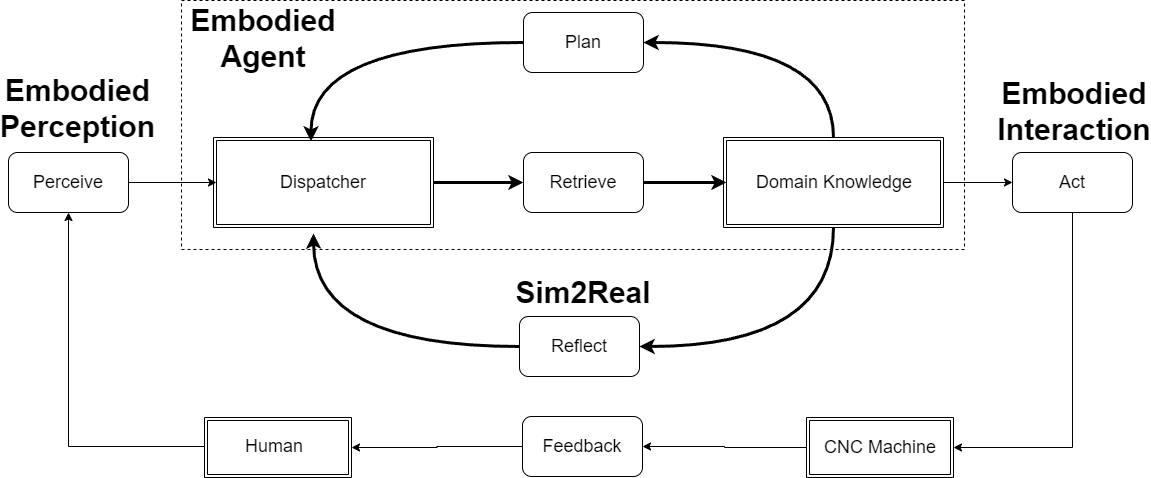
\includegraphics[width=0.8\linewidth]{1.png}
    \caption{Emerging Demands in Intelligent Manufacturing}
    \label{fig: Fig.1}
\end{figure}

As highly integrated electromechanical devices, NC machine tools feature precise control of servo systems and complex trajectory interpolation operations as one of their core technologies\cite{liu2023feedrate}. Servo systems play a crucial role within NC machine tools, using servo motors, amplifiers, and feedback devices to precisely control the machine's motion position, speed, and acceleration, ensuring high accuracy and stability during the machining process. These systems are particularly suited for producing diversified, high-precision, small-batch parts\cite{luo2020hybrid,zhong2020toolpath}. With the development of information and communication technologies, NC machine tools are transitioning from closed to open architectures, gradually increasing their frequency of use in manufacturing workshops\cite{liu2023open,deng2018open}. In the broader context of interconnectedness, the integration of emerging technologies such as the Internet of Things (IoT), artificial intelligence, and edge computing further promotes the intelligence of servo systems, enabling NC machine tools to achieve a more flexible and efficient manufacturing loop, as illustrated in Figure 2. The enhancement of servo systems, coupled with using sensors and edge computing devices, endows NC machine tools with self-perception, self-adjustment, self-prediction, and self-assessment capabilities\cite{ye2020knowledge}. This not only augments the functionality of NC machine tools but also expands their application domains. Furthermore, intelligent NC systems are responding to the following new industrial development demands:

\begin{enumerate}
    \item With the evolution of intelligent manufacturing, NC systems must break down information silos to achieve efficient interconnectivity between devices.

    \item The deluge of data by IoT technologies and the stringent demands for real-time processing pose new challenges to NC systems' immediate data handling and response capabilities.

    \begin{figure}[h]
        \centering
        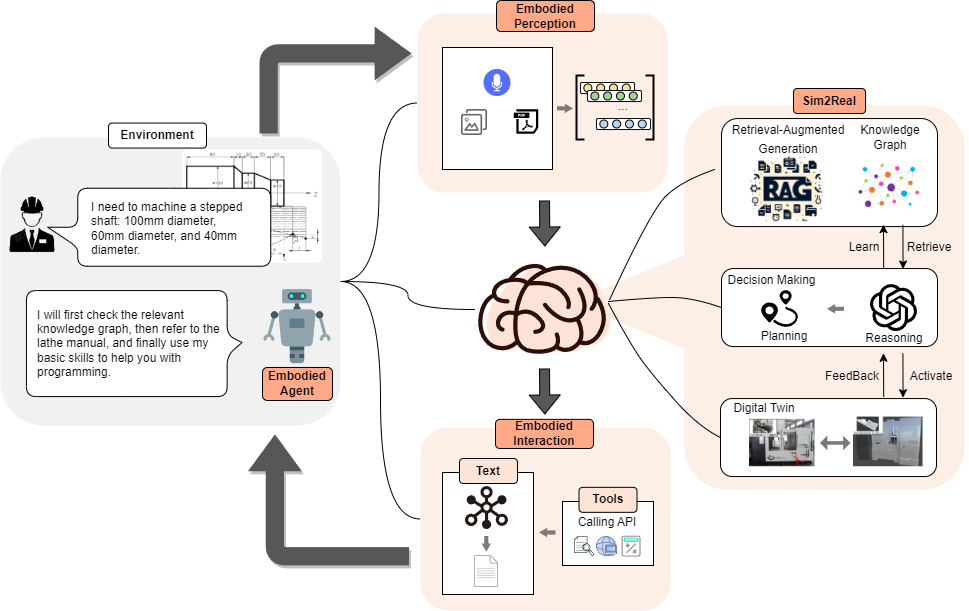
\includegraphics[width=\linewidth]{2.png}
        \caption{Intelligent NC System with Adaptive Control}
        \label{fig: Fig.2}
    \end{figure}

    \item Given the importance of data privacy protection, especially in high-end manufacturing sectors like aerospace, industrial producers are cautious about cloud data processing, preferring local processing and storage of critical information.

    \item The limited resources of industrial sites, along with the pursuit of production accuracy, quality, and efficiency, require servo systems to enhance the production throughput of NC machine tools while ensuring machining precision.
    
\end{enumerate}

\subsection{System Modeling and Structure}
A modular structure plays a pivotal role in the design of numerical control systems. When it comes to the intelligentization of these systems, such an architectural approach enhances their adaptability and scalability and lays a solid foundation for real-time monitoring and operational precision\cite{yu2023edge}.


Within the modular construction of numerical control systems, the synergy between various intelligent elements across modules fosters a dynamic environment for learning and self-optimization, as illustrated in Figure 3. This interplay significantly bolsters the system's adaptability and autonomy. The intelligent elements include:

\begin{itemize}
    \item Perception and Interconnectivity: Sensing the state and environment of the numerical control system through sensors and other data acquisition methods. This information forms the foundation of the intelligent system's decision-making and must be accurately collected and processed.

    \item Digital Twin Models: Virtual replicas of the physical numerical control systems that can simulate and analyze system performance in real time. Through this mechanism, intelligent systems can anticipate future states or understand the potential impacts of specific actions.

    \item Learning and Modeling: The capability of the intelligent system to learn from its current state and model the situation accordingly. This involves employing deep learning algorithms to identify patterns or anomalous behaviors to assess the system's operational status or maintenance needs.

    \item Optimization and Decision Making: Based on the assessment and diagnosis of the current state, the intelligent system must be able to make decisions and execute actions for optimizing tasks. This could involve adjusting system parameters, initiating maintenance procedures, or altering operational strategies to enhance efficiency and performance.
\end{itemize}

This process manifests in intelligent numerical control systems as continuous data collection by various modules (such as machine status, machining efficiency, and motor positions) to adjust strategies for optimizing system performance. The effectiveness of these improvements is then validated through actual machining outcomes. This cycle ensures that the numerical control systems can self-optimize and adapt to evolving production demands.

\begin{figure}[hbt]
    \centering
    \includegraphics[width=\linewidth]{3.png}
    \caption{Intelligent Elements Modeling Scheme of NC Systems}
    \label{fig: Fig.3}
\end{figure}

In intelligent manufacturing, numerical control systems perform numerous critical functions, such as intelligent monitoring and optimization in synchronous control and trajectory planning for NC machine tools. These functions demand stringent time controls to ensure machining accuracy and efficiency. Under traditional cloud computing models, limitations in network bandwidth and latency could lead to uncertainties in timing delays, affecting the timeliness of real-time data processing and potentially leading to discrepancies between the physical machine tools and their digital twins\cite{liu2023intelligent,xiao2024step}. Adopting edge intelligence methods becomes an essential solution strategy to address this issue, significantly reducing the time required for data transmission and processing by processing data near its source, thereby ensuring data interaction consistency and synchronicity\cite{nain2022towards}. This technology is indispensable for the real-time and accurate execution of numerical control systems. In this context, we have constructed a comprehensive intelligent data processing architecture, as shown in Figure 4. This layered and modular approach enhances the system's flexibility, providing robust technical support for numerical control systems within an intelligent manufacturing environment.

Physical Layer: Primarily consists of NC machine tools and various sensors, acting as the data source, responsible for real-time capture and monitoring of machine operation data. Continuous monitoring of machine states by these sensors collects critical performance parameters. It uploads this raw data directly to the network layer, ensuring comprehensive and timely data collection for precise input to higher-level processing.

Network Layer: Edge nodes and servers within this layer form the vanguard of data processing, undertaking data relay, preliminary processing, and intelligent analysis. Positioned close to the physical sources, edge nodes can preprocess collected data, such as data cleansing and preliminary analysis, to alleviate the load on the cloud. Edge servers further process this data, running advanced algorithms for process optimization, machining simulation, health management, and establishing digital twins, providing essential support for real-time decision-making. This layer's design makes data processing more efficient and responsive, offering immediate and reliable information support for the application layer.

Application Layer: Users access real-time monitoring, fault prediction, and diagnostic services through interactive interfaces connected to the network layer's cloud and edge computing resources. This layer not only presents the analytical outcomes of the network layer but also integrates advanced data processing from the cloud with the immediate decision-making capabilities of edge computing, achieving intelligent control of the production process. Furthermore, through close cooperation with the cloud and edge layers, the application layer can offer rapid feedback and decision support, enhancing the system's autonomy and production efficiency.

\begin{figure}[hbt]
    \centering
    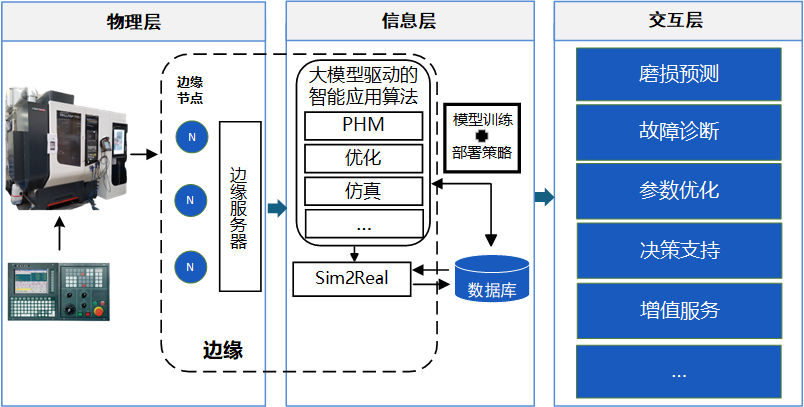
\includegraphics[width=\linewidth]{4.png}
    \caption{Network Topology Diagram}
    \label{fig: Fig.4}
\end{figure}

The real-time perception and processing of data are paramount within the intelligent architecture of numerical control systems.  By deploying various sensors, such as vibration, sound, and temperature sensors, on CNC machine tools, the system facilitates immediate data capture, transmitting it to edge nodes.  Once set with appropriate collection frequencies, these nodes are tasked with data acquisition and preliminary preprocessing.  These nodes communicate with intelligent gateways on edge servers through WebSocket protocols while utilizing GB/T39561\cite{GT3956142020} and OPC UA protocols to handle data from the numerical control systems, ensuring rapid transmission and high data accuracy.  Edge servers, via intelligent gateways, integrate multiple communication protocols, allowing multiple nodes to connect as clients and store information in the GB/T39561 data format compliance using the OPC UA modeling approach, facilitating data subscription and further processing.

In the edge computing architecture, the KubeEdge platform plays a pivotal role, integrating edge servers and nodes under the unified management of the cloud-based Kubernetes cluster. CloudCore in the cloud is responsible for task distribution and scheduling, whereas EdgeCore at the edge ensures local task execution and management\cite{kundroo2022node,kim2023local}. Through containerization, components of neural network models can run efficiently on the most suitable edge computing resources and synchronize with the cloud, maintaining harmony and coordination. This distributed computing structure not only enhances execution efficiency but also guarantees quick responses to real-time data processing. Moreover, customized communication protocols support effective collaboration between edge devices, augmenting the flexibility and response speed of the entire intelligent manufacturing system, thereby bolstering the performance of edge computing.

\subsection{Functional Subcomponents and Model Construction}

\subsubsection{Edge Computing Infrastructure Design}

In the contemporary design of edge computing infrastructure, Figure 5 unveils a modular architecture for the intelligent data processing of numerical control system information, seamlessly integrating the processes of data acquisition, analysis, and application decision-making. Within the perception module, the numerical control system utilizes CNC controllers, sensors, and servo systems to monitor various operational metrics of the machine tools in real time. Specific attribute data (such as machine status, operational model, and G-code line numbers) are directly connected to the edge server through DLL or industrial communication protocols like MQTT and Modbus; other data (such as vibration signals from the X, Y, and Z axes) require initial transmission to an edge node, where they undergo preprocessing before being relayed to the edge server.

Leveraging the high-performance computing capabilities of the NVIDIA Jetson Xavier NX, the edge server conducts preliminary parsing and structuring of data, facilitating subsequent analysis. The edge server module is designed with modularity in mind to handle various complex analysis tasks adeptly. Guided by information and mechanistic models, this module employs efficient data fusion, analysis, and storage strategies in conjunction with application algorithms, executing advanced algorithms such as tool path optimization to assess the current state of machine tools and predict future maintenance requirements. These analytical outcomes are then instantaneously fed back into production process decisions through the control logic module, ensuring the optimization of operations and maximization of machine tool performance.

The proposed architecture's edge intelligence-based numerical control system model provides critical support for achieving intelligent objectives. This design optimizes dynamic task allocation between edge servers and computing nodes, ensuring the timeliness and efficiency of proximal data processing and effectively alleviating the cloud processing load. By allocating tasks with high immediacy requirements to be executed on edge computing nodes, processing speed is enhanced, and resource allocation is optimized, rendering the design of edge computing infrastructure more efficient and responsive.

\begin{figure}[hbt]
    \centering
    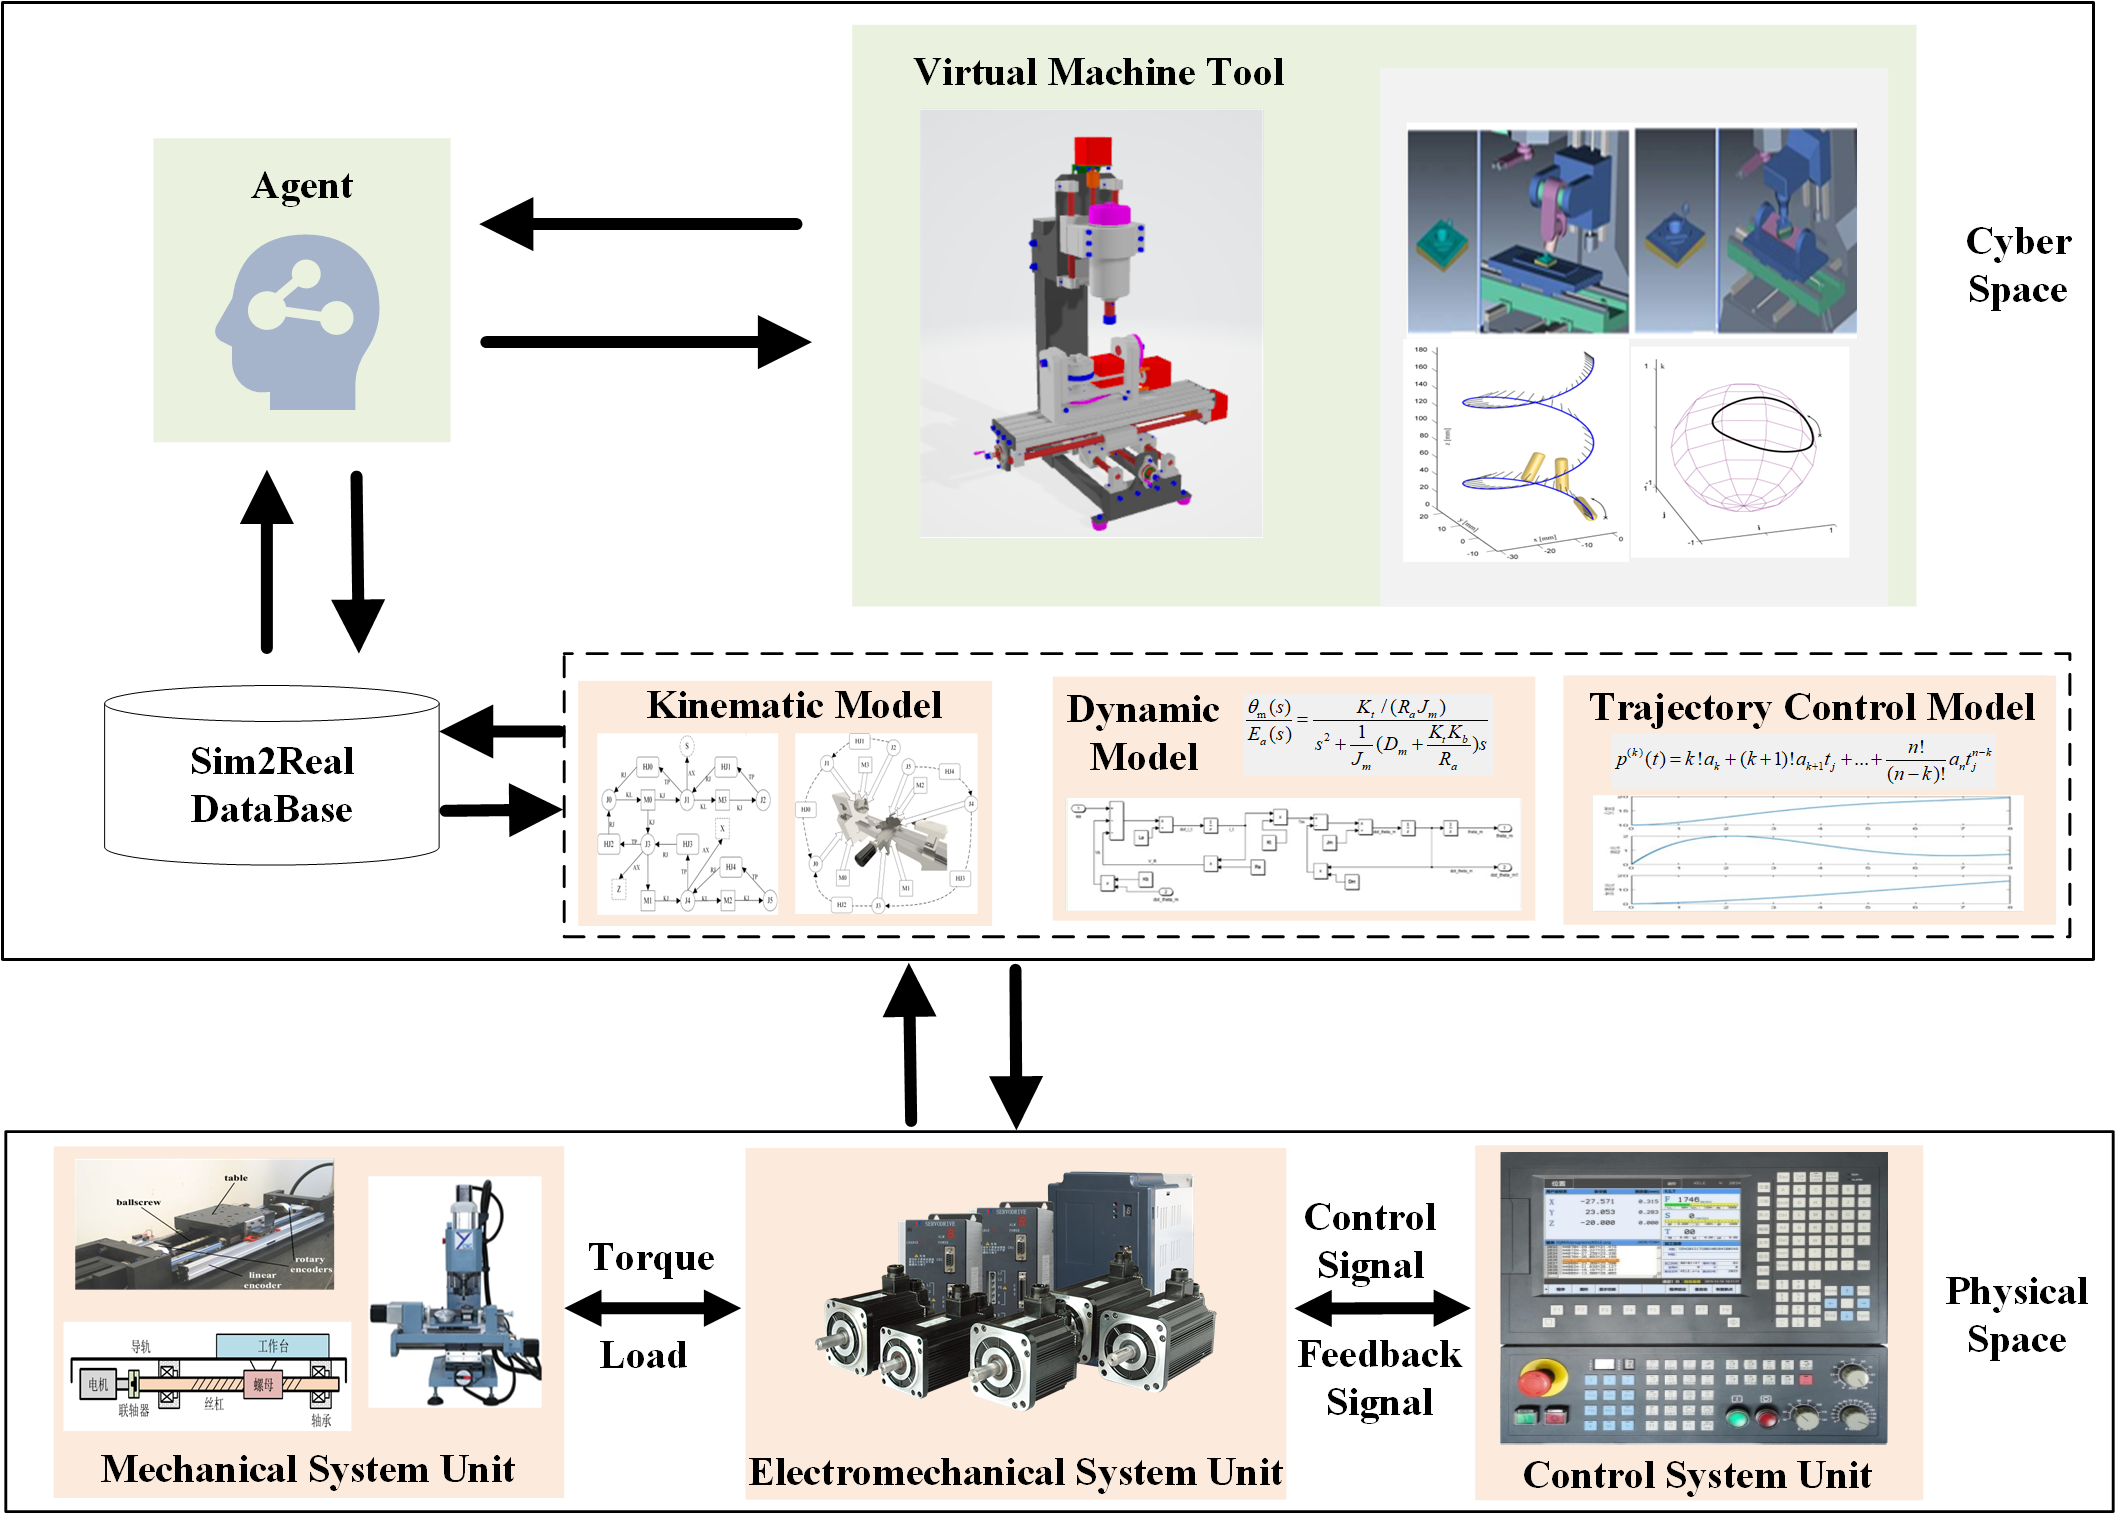
\includegraphics[width=\linewidth]{5.png}
    \caption{Edge Intelligence-Based NC System Structural Model}
    \label{fig: Fig.5}
\end{figure}

\subsubsection{Construction of Information Model (IM) and Mechanistic Model (MM)}

In modern numerical control systems' intelligent and networked architecture, reliance on precise and efficient Information Models (IM) and Mechanism Models (MM) is essential for real-time monitoring and effective management. We can significantly enhance model accuracy and system response efficiency by adopting standardized modeling and simulation techniques, thereby meeting the performance requirements in an edge intelligence environment.

\textbf{Construction of Information Model (IM)}

In constructing the Digital Twin's Information Model (IM) for numerical control systems, the systems themselves and data acquisition devices play a crucial role. Following the GB/T 39561.4-2020 standard, we have conducted a comprehensive analysis of the basic information model of CNC equipment, encompassing static attributes (describing inherent system characteristics), process attributes (reflecting operational characteristics of the system), configuration attributes (necessary configurations for executing tasks), and various components (such as CNC controllers, servo systems, I/O, PLCs, etc.). These elements collectively support the real-time monitoring and efficient management of the numerical control system, as depicted in Figure 6.

\begin{figure}[hbt]
    \centering
    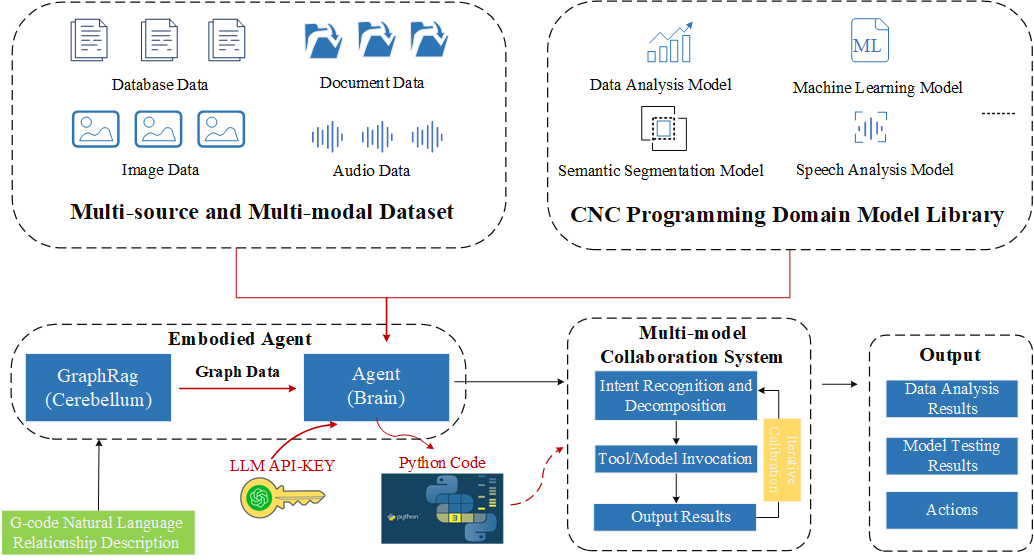
\includegraphics[width=\linewidth]{6.png}
    \caption{Information Model of NC System}
    \label{fig: Fig.6}
\end{figure}

\textbf{Construction of Mechanism Model (MM)}

In precision manufacturing processes, achieving accurate control across multiple axes of CNC machine tools is paramount, directly impacting production precision and efficiency. However, traditional control methods that rely on mechanical adjustments face significant challenges in addressing the non-linearity and dynamic changes during machining processes\cite{youssef2023review,you2021adaptive}. Due to slow response times, these methods often fail to compensate effectively for machining inaccuracies and diminished machine performance. This limitation primarily arises from the traditional control devices' lack of adaptability to real-time changes in machining conditions and mechanical wear; moreover, these control methods are designed for linear systems and do not align with the non-linear dynamical characteristics of CNC machinery. Additionally, there is a noticeable delay in responding to dynamic changes due to slow processing and reaction times. These limitations underscore the constraints of traditional methods in modern precision manufacturing and highlight the necessity of adopting more advanced control strategies to overcome these challenges.

These limitations accentuate the demand for more advanced, intelligent methods. The choice of neural network-based control and monitoring is primarily due to neural networks' ability to handle complex non-linear issues in CNC system operations, especially in scenarios of synchronous control. Unlike traditional control methods, neural networks can learn and identify complex patterns and relationships from data, providing more accurate and dynamic control strategies. This method not only adapts to subtle changes in system behavior but also processes and responds in real-time, ensuring the high precision and efficiency of CNC systems. Furthermore, the real-time monitoring capabilities supported by neural networks continuously optimize operational parameters, reduce manual intervention, and enhance automation levels. Thus, neural network-based monitoring and optimization are ideal for addressing synchronous control issues.

\begin{figure}[hbt]
    \centering
    \includegraphics[width=0.75 \linewidth]{7.png}
    \caption{Edge Intelligence-Based Synchronous Control Monitoring and Optimization Process}
    \label{fig: Fig.7}
\end{figure}

To address the challenges of synchronous control in high-speed, high-precision machining encountered by CNC systems and to overcome the limitations of traditional control methods in handling non-linear dynamic systems, this study employs an advanced model based on deep neural networks. Leveraging their exceptional non-linear modeling capabilities and adaptive learning features, the model can effectively learn optimal strategies for synchronous control from complex currents, speeds, and positional data, as shown in Figure 7. In this process, the neural network plays a crucial role, accurately predicting the CNC system's dynamic error adjustment needs in real time and automatically optimizing control parameters based on these predictions, thereby achieving high-precision dynamic error compensation. Deploying this deep neural network model on edge computing devices enables real-time monitoring and optimization of CNC systems, significantly enhancing machining efficiency and product quality. The model's feedback learning mechanism also ensures the system can continuously adapt to new working conditions and wear states, maintaining long-term high-performance operation. This approach strengthens the response capability to dynamic changes and enhances the system's adaptability and flexibility, showcasing the immense potential of deep learning-based control strategies in modern precision manufacturing.

To ensure high-precision synchronous control of CNC systems in complex machining environments, this study introduces a set of anomaly detection and adjustment strategies based on deep neural networks. Initially, the calculation formula for anomaly detection thresholds can be expressed as:

\begin{equation}
    G=|P_{actual}-P_{expected}|
    \label{equation:1}
\end{equation}

Equation \ref{equation:1} quantifies the deviation between the actual and expected positions, where D represents the dynamic error between these two points. When this error exceeds a predetermined threshold θ, it is identified as an anomalous state requiring control adjustment. The threshold θ is based on analyzing historical data and understanding mechanical performance, aiming to find a balance between the system's response sensitivity and operational practicality.

Furthermore, to execute the necessary adjustments with precision, this study utilizes an adjustment calculation formula as follows:

\begin{equation}
    A=S \times G
\end{equation}

The adjustment amount A, calculated through Equation 2, directly correlates with the actual adjustment actions the system needs to undertake to ensure optimal outcomes. Here, S acts as a sensitivity factor, adjusting the proportion of the adjustment amount based on the magnitude of dynamic error D, allowing the system to respond flexibly under actual operational conditions. This strategy enhances the NC system's ability to handle nonlinear issues. It improves adaptability and precision when facing complex machining tasks, ensuring high consistency between machining efficiency and product quality.

\subsection{Edge Intelligence-Based Model Deployment Method}

In the realm of numerical control systems, the deployment of models based on edge intelligence is achieved through a series of meticulously orchestrated steps. As illustrated in Figure 8, initially, upon sensing data from the numerical control system, edge nodes identify available computing resources through service discovery, laying the groundwork for subsequent operations. In the neural network task segmentation phase, complex deep learning models are divided into multiple neural network subtasks, maintaining the functional integrity of each segment to facilitate effective execution across various computing environments. Intelligent offloading decisions are made based on task latency and throughput metrics, automatically selecting whether to offload to high-performance devices and which subtasks to offload. The task transmission phase involves securely and efficiently transferring selected tasks to the designated computing devices. These devices then undertake the responsibility of computation execution, processing the tasks allocated to them. Ultimately, the processed results are relayed back to the edge nodes to be fed back into the production process or for further analysis, thereby completing a cycle of model deployment based on edge intelligence.

\begin{figure}[hbt]
    \centering
    \includegraphics[width=0.5\linewidth]{8.png}
    \caption{Fundamental Process of Computational Offloading in NC Systems}
    \label{fig: Fig.8}
\end{figure}

Within our edge intelligence-based numerical control system application model deployment environment, we define a computation offloading problem to optimize task processing latency and resource utilization. They are considering a set \(N\), where \(N=\{N_i |i=1,2,...,n\}, N_i\) represents an independent neural network subtask and a total of n subtasks; these subtasks must be processed on the intelligent numerical control system's edge nodes or edge servers. Each subtask requires a decision on whether its computation must be offloaded to the edge server. To align decision outcomes closer to achieving an optimal task offloading partitioning that balances latency, throughput, and latency threshold, a mathematical model is introduced into the environment as part of the reward, aiming to maximize subtask real-time strategy performance and optimal allocation of computing resources under the oversight of the observer. Offloading decisions must consider the dependencies between tasks, the dynamic nature of network conditions, and each neural network layer's computational and data transmission requirements, simultaneously flexibly improving the original approach that solely relied on a one-size-fits-all mathematical model.

\subsubsection{Resource Allocation Optimisation Modeling}

In edge intelligence-based numerical control systems, modeling for optimizing network and computing resource allocation is a critical component in reducing service latency and ensuring service quality. In our offloading environment, we model different resource allocation optimization models involving network and computation.

\textbf{Network Resource Allocation Optimisation Model}

Under the "cloud-edge-device" architecture, each edge node can process each subtask locally or offload the computational task to the edge server through the channel. The computation offloading strategy for subtasks within edge nodes can be defined as follows:

% \begin{equation}
%     a_i\left\{
%         \begin{aligned}
%             &0,&Local \ Computing\\
%             &1,&Local \ Offloading
%         \end{aligned}
%     \right.
% \end{equation}

\begin{equation}
a_i = \left\{
    \begin{aligned}
        &0, && \text{Local Computing} \\
        &1, && \text{Local Offloading}
    \end{aligned}
\right.
\end{equation}

Thus, \(a_n=(a_1,a_2...,a_n)\) represents the set of all subtask computation offloading strategies for the edge node.

Based on the Shannon capacity formula, the uplink transmission rate during the offloading of computational tasks from edge nodes to edge servers is

\begin{equation}
    C_{i,up}(a_i)=Klog_2(1+S_{i,up}/N_i)
\end{equation}

Similarly, the downlink transmission rate is

\begin{equation}
    C_{i,down}(a_i)=Klog_2(1+S_{i,down}/N_i)
\end{equation}

Within this context, \(K\) represents the bandwidth between the edge node and the server. For \(S_{i, up}=q_{i, up}g_{i, up}\) and \( S_{i, down}=q_{i, down} g_{i, down}, q_{i\\, up}\) and \(q_{i, down}\)  denote the transmission power of the edge node and edge server, respectively, while \(g_{i, up}\) and \(g_{i, down}\) correspond to the uplink and downlink channel gains. \(N_i=\sigma+\sum_{i\in{N}:a_i=a_n}q_i g_i\), where  \(\sigma\) represents the background white noise interference, and  \(\sum_{i\in{N}:a_i=a_n}q_i g_i\) signifies the communication interference from other channels. The uplink and downlink rates are defined as the maximum throughput in the network transmission task, allowing the channel capacity derived from the Shannon formula to be considered as the maximum possible throughput for this network transmission task.

\textbf{Computational Resource Allocation Optimization Model}

The computational resource allocation optimization model has two modes: edge node computation and edge server computation. The computation-intensive tasks at the edge node can be defined as \(I_i \triangleq B_i\), where \(B_i\) represents the volume of data required by the edge node to complete the computation task.

\begin{itemize}
    \item {\fontsize{11}{\baselineskip}\selectfont \textbf{Edge Node Local Computation}}
\end{itemize}

When the computation results from the edge server need to be transmitted back to the edge node, the edge server transmits the results to the edge node through the channel, defining the time cost of the download transmission process as:

\begin{equation}
    t_{i,down}^{edge} (a_n )=\frac{B_i}{C_{i,down} (a_n )} 
\end{equation}


When the decision is for the edge node to compute locally, subtask i is executed on the edge node to perform computation task \(I_i\). Let \(f_i^edge\) represent the computational capability of the edge node (i.e., the CPU clock frequency in Hz). Thus, the execution time for performing computation task \(I_i\) on the edge node is:

\begin{equation}
    t_{i,exe}^{edge}=\frac{B_i}{f_i^{edge}}
\end{equation}

The total cost of computation at the edge node is:

\begin{equation}
    K_n^{edge} {a_n}=\lambda_n^t (t_{n,down}^{edge} (a_n )+t_{n,exe}^{edge} )
\end{equation}


Here, \(\lambda^t_n \in (0,1)\) denotes the computational time weight assigned by edge node n at the decision-making time. It sets the value based on the sensitivity requirement to latency in its scenario, thereby dynamically adjusting the system's overall cost.

\begin{itemize}
    \item {\fontsize{11}{\baselineskip}\selectfont\textbf{Edge Server Computation}}
\end{itemize}

When the edge node decides to compute at the edge server, the edge node offloads the computation-intensive task to the edge server through the channel, defining the time cost of the offloading transmission process as:

\begin{equation}
    t_{i,up}^{server} (a_n )=\frac{B_i}{C_{i,up} (a_n )} 
\end{equation}

The computational capability of the edge server, represented by the clock frequency \(f_n^c\), then the time to execute computation task \(I_n\) is:

\begin{equation}
    t_{i,exe}^{server}=\frac{B_i}{f_i^{server}}
\end{equation}

The total cost of computation at the edge server is:

\begin{equation}
    K_n^{server} {a_n}=\lambda_n^t (t_{n,up}^{edge} (a_n )+t_{n,exe}^{server} )
\end{equation}

Here, \(\lambda_n^t\in(0,1)\). Since many offloaded computation-intensive tasks involve a large volume of computational input data. In contrast, the computational feedback results are often minimal, and the time cost of feedbacking the computation results to the edge node can be disregarded.

\subsection{Evaluation Method Based on Integer Linear Programming (MILP)}

Task partitioning is the pivotal step in the evaluation. It aims to identify the optimal division point that balances latency and throughput, allocating tasks before the partition point to the edge node and tasks after it to the edge server\cite{wang2023task}. We employ Mixed Integer Linear Programming (MILP) to address this challenge.

Specifically, the steps for task partitioning are as follows:

\begin{enumerate}
    \item Create a MILP problem with an objective function that aims to minimize the total delay variance, thus combining the effects of delay and throughput. This can be expressed in the following equation:

    \begin{equation}
        latency_{diff}=\sum^n_{t=1}|(t_{i,exe}^{edge}-t_{i,exe}^{server})\cdot y_i|
    \end{equation}

    Here, \(n\) denotes the number of tasks, \(t_{i,exe}^{edge}\) and \(t_{i,exe}^{server}\), respectively, signify the execution times of task \(i\) on the edge node and edge server, and \(y_i\) is a binary decision variable indicating whether task \(i\) is partitioned after that.

    \item Introduce constraints to ensure the total latency does not exceed an acceptable threshold. These constraints consider the latency of each task on edge devices and cloud servers and data transmission latency. The specific constraints are as follows:

    \begin{equation}
    latency_i^{edge}=\sum^i_{j=1}t_{j,exe}^{edge}+t_{i,up}^{server}(a_n)
    \end{equation}

    \begin{equation}
        latency_i^{server} = \sum^n_{j=j+1}t_{j,exe}^{server}+N\cdot t_{i,down}^{edge}(a_n)
    \end{equation}
    
    \begin{equation}
        latency_i^{edge}\cdot y_i+latency_i^{server}\cdot(1-y_i)\leq latency_{tolerable}
     \end{equation}

    Here, \(latency_i^{edge}\) and \(latency_i^{server}\) represent the latency of task \(i\) on the edge device and edge server, respectively, \(t_{i,up}^{server}(a_n)\) and \(t_{i,down}^{edge}(a_n)\) denote the data uplink and downlink transmission latency of task \(i\), and \(latency_{tolerable}\) is the acceptable total latency threshold.
    
\end{enumerate}

Ultimately, by solving the MILP problem, we obtain the optimal task partition point regarding latency and throughput, along with other crucial information related to the partition, such as total latency, latency on the edge nodes and edge servers, data transmission latency, throughput, etc., thereby deducing the optimal partition point based on latency and throughput.

\section{Design and Application of Intelligent CNC System Offloading Algorithm Based on Reinforcement Learning }

Within the framework of numerical control systems based on edge intelligence, the design and application of Artificial Intelligence (AI) algorithms, particularly methods of Reinforcement Learning (RL), play an essential role. Reinforcement Learning, characteristic of self-exploration and learning, offers unique advantages in addressing the dynamic and uncertain issues within numerical control systems. This section delves into the design and application of algorithms based on reinforcement learning, detailing their implementation in task-offloading strategies and system performance optimization.

\subsection{Task Offloading}

Task offloading, a central issue in edge computing scenarios, involves transferring computationally intensive tasks from resource-constrained edge nodes to more resource-abundant servers to enhance computational efficiency and reduce latency. A practical task offloading strategy is crucial for achieving real-time monitoring and optimization in numerical control systems powered by edge intelligence.

\textcolor{red}{在我们的数控系统中，基于强化学习的任务卸载算法调用是建立在对系统性能指标的精细观察与分析基础之上的。当数控系统面临资源分配的挑战，如计算资源竞争加剧或任务处理需求迅速变化时，我们便考虑利用强化学习进行优化决策。我们设定了几个关键指标作为触发强化学习调用的信号。其中，最直观的指标是任务等待时间与系统处理能力的比值，当该比值超过预设的阈值，比如超过系统平均处理能力的20\%，表明系统正面临较大的处理压力，需要通过强化学习来优化任务卸载策略，以减轻延迟和提高资源利用效率。此外，数据传输速率与处理速率的差异也是一个重要的考量因素；当观察到数据传输延迟占整体任务处理时间的比重显著上升，达到或超过30\%，说明网络状态可能对任务执行效率产生了较大影响，这时强化学习算法将被调用来重新评估并优化数据流和计算任务之间的调度策略。通过量化指标的方式，我们能够在系统运行过程中准确地识别出何时需要借助强化学习的能力，以实现更高效、更灵活的数控系统运行策略。}

\textcolor{red}{在强化学习被调用以优化数控系统任务卸载的整个过程中，系统状态的持续监测是起点，包括实时收集系统的计算负载、网络带宽利用率及任务队列长度等关键性能指标。达到预设的触发条件后，自动进入数据采集阶段，此时涉及收集与当前任务相关的数据，例如任务类型、资源需求和预期完成时间，为决策评估提供所需信息。基于这些数据，强化学习模型评估当前的任务卸载策略，通过计算预期奖励值来衡量策略效果。此评估结果指导模型学习，并更新决策策略，包括调整策略参数以最大化长期奖励。这一更新策略随后应用于实际任务卸载决策，旨在减少延迟、提升处理速度和提高资源利用率，确保数控系统能够自动调整策略，适应不断变化的系统运行状况，维持最优性能。}

\textcolor{red}{强化学习模型的训练采用了测量神经网络的历史运行数据，利用从子任务的过往运行中累积的大量计算任务执行结果、网络状况及任务处理时间等数据，训练模型以识别和学习最有效的任务卸载策略。通过这种方法，模型能够在不同的系统状态下预测最优的任务卸载决策，以此来最小化执行延迟并提高系统效率。训练完成后，该模型被集成进数控系统的边缘计算层，使得它能够实时监测系统状态，并根据当前的环境和系统性能，动态地调整任务卸载策略。这种集成不仅提升了系统的自适应能力，使其能够在面对不断变化的工作负载和网络条件时保持高效运行，同时也确保了系统能够从每一次任务执行中学习并不断优化其决策过程，确保智能化数控系统在保持高性能的同时，也最大化地利用了可用资源。}

The task initiation phase involves evaluating the computational performance of edge nodes and servers and reviewing designated subtasks. For a data processing task composed of \(n\) subtasks, the system calculates the execution latency of each subtask \(i\) on the edge nodes (\(latency_i^{edge}\)) and the edge servers (\(latency_i^{server}\)) based on theoretical formulas from section 3.4. Since subtasks' processing delay primarily depends on the hardware's computational performance, a one-time latency initialization is sufficient for similar hardware devices. The execution delay of each subtask \(i\) can be determined based on the actual operating performance of the hardware.

The collaborative computing offloading framework based on reinforcement learning proposed in this section aims to dynamically optimize task offloading strategies to adapt to the real-time operational status and changing network environments of numerical control systems. In this framework, an agent is responsible for processing neural network layers and, based on observations such as environmental bandwidth, inference latency of edge nodes and servers, and the actions of previous subtasks, determines the optimal model partitioning decision and pruning weight distribution through a reward function. As illustrated in Figure 9, the system, guided by the agent's decisions, divides the original neural network model into several subtasks. Since solely relying on reinforcement learning for offloading decisions of each subtask might lead to frequent data transmission between closely related tasks, thus increasing the acceptable total latency threshold, the Actor-Critic mechanism is used to assess the decisions, seeking the optimal division method to distribute tasks between edge nodes and servers effectively. This ensures the overall runtime latency remains within acceptable limits, optimizes latency and throughput, and improves the traditional "one-size-fits-all" task partitioning approach. Determining the optimal partitioning strategy is a complex process that depends on the structure of the neural network, the computational capacity of hardware devices, network conditions, and mathematical methods tuned to maximize total rewards. This framework demonstrates how continuous learning and strategy adjustments can optimize response times and computational efficiency in changing operational environments.

\begin{figure}[hbt]
    \centering
    \includegraphics[width=\linewidth]{9.png}
    \caption{Collaborative Computing Offloading Method Based on Reinforcement Learning}
    \label{fig: Fig.9}
\end{figure}

\subsection{Intelligent Agent Interaction Environment Design}

Designing a reinforcement learning algorithm framework suitable for task offloading in numerical control systems is foundational for achieving real-time monitoring and optimization. This section focuses on constructing a reinforcement learning algorithm framework suitable for task offloading in numerical control systems, detailing the agent's interactive environment, including precisely defined state space, action space, reward function, and state transition dynamics.

In the environmental state, the \textbf{State Space} is defined as a multi-dimensional feature set reflecting the current subtask. For the \(i\)th subtask, the state \(s_i\) is represented as:

\begin{equation}
    s_i=[c_i,d_i,i_i,q_i,a_{i-1},a_{i-2} ]
\end{equation}

Here, \(c_i\) represents the computational demand of the current subtask \(i,d_i\) describes the data transmission requirement, \(i_i\) is the current task's index in the queue, \(q_i\) is the number of remaining tasks in the queue, and \(a_{i-1}\) and \(a_{i-2}\) is the action selections of the two preceding tasks. This comprehensive state representation gives the agent a complete environmental view, enabling more informed decision-making.

The \textbf{action space} is set as two discrete options:

% \begin{equation}
%     \label{eq:17}
%     \left\{
%         \begin{aligned}
%             &a_i=0, &Executing\ the \ i^{th}\ subtask \ on \ the\ edge\ node\\
%             &a_i=1, &Executing\ the \ i^{th}\ subtask \ on \ the\ edge\ server
%         \end{aligned}
%     \right.
% \end{equation}

\begin{equation}
    \label{eq:17}
    \left\{
        \begin{aligned}
            &a_i=0, && \text{Executing the } i\textsuperscript{th} \text{ subtask on the edge node}\\
            &a_i=1, && \text{Executing the } i\textsuperscript{th} \text{ subtask on the edge server}
        \end{aligned}
    \right.
\end{equation}



This binary choice of action space is designed to simulate a simplified scenario of task-offloading decisions in the real world.

We designed a composite \textbf{reward function} \(R(s_i,a_i)\) incorporating several vital factors to guide the agent toward learning the optimal task offloading strategy. This function considers the latency of task execution (unified here as \(L_i\) for both \(latency_i^{edge}\) and \(latency_i^{server}\))  and throughput (unified here as \(C_i\) for both \(C_{i, up} (a_i)\) and \(C_{i, down} (a_i)\)), along with the cost of action and the Critic's evaluation.

\begin{itemize}

    \item {\fontsize{11}{\baselineskip}\selectfont \textbf{Latency and Throughput Trade-off}}: Initially, latency and throughput are calculated based on the location of task execution (either at the edge node or edge server). The reward function incorporates a trade-off between minimizing latency and maximizing throughput. After normalization, the reward is calculated using the following equation:

        \begin{equation}
            R_i=\alpha log(L_i+1\times 10^{-3})+(1-\alpha)log(C_i+1\times 10^{-3})
        \end{equation}

    \textcolor{red}{其中，\(\alpha\)是一个权衡参数，用于平衡延迟和吞吐量在奖励中的重要性。我们在考虑奖励函数时，采用对数函数（log）主要基于其非线性响应特性。这种调节方式对小规模的延迟和吞吐量变化极为敏感，而对大规模变化反应平缓，使得模型在微小的性能变化中展示出较高的反应灵敏度，同时在极端值出现时保持稳定性，有利于策略的细致学习和优化。对数函数通过自然的曲线形态有效地平滑处理极值情况，避免了使用延迟或吞吐量的倒数可能导致的奖励值大幅波动，确保奖励函数的稳定性和计算的可靠性。此外，该函数形态在延迟减少和吞吐量增加时能够提供正向的奖励强化，与优化目标—即最小化延迟和最大化吞吐量—保持一致。为了数学上的稳定性，我们引入了一个小常数\(1.0*10^3\)以避免函数输入值为零的情况，确保函数在整个定义域内的良好行为和操作的安全性。}

    \item {\fontsize{11}{\baselineskip}\selectfont \textbf{Critic evaluation}}: To increase the diversity of the agent's strategies and introduce external knowledge, our reward function also includes a section based on Critic evaluation. Critic evaluation adjusts the reward based on the degree of alignment between the agent's actions and predefined recommendations.
    

\end{itemize}

The \textbf{State Transition Dynamics (STD)}  are determined based on the current state, actions taken, latency, and throughput. The specific formula is as follows:

\begin{equation}
        s_{i+1}=f(s_i,a_i,L_i,C_i,I_{i+1},q_{i+1})
    \end{equation}

Here, \(f\) represents the state transition function, combining the current state \(s_i\), action \(a_i\), and the latency \(L_i\) and throughput \(C_i\) induced by the action, and updates the task index \(indexI_(i+1)\) and queue length \(q_{i+1}\).

\subsection{Evaluation Algorithm Design}

The task offloading algorithm presented in this paper is designed to efficiently allocate tasks between edge devices and servers to minimize total latency while maximizing throughput. The crux of the algorithm encompasses task partitioning and partition recommendations, coupled with the introduction of Critical evaluation to further refine the agent's decision-making process.

\textbf{Partition Recommendations}

Partition recommendations form a segment of the algorithm aimed at advising the optimal execution location for each task—whether on the edge node or edge server. Utilizing the optimal partition point obtained in the task partitioning step, a suggestion for each task is provided, as depicted in Equation \ref{eq:17}. This results in constructing a binary list, where each element indicates the recommended execution location for the corresponding task. For instance, if the \(i\)th element of the recommendation list is '0', task i should be executed on an edge device; if it is '1', task i should be carried out on a cloud server.



\RestyleAlgo{ruled}
\SetKwComment{Comment}{/* }{ */}

\begin{algorithm}[H]
    \caption{Reward Calculation Algorithm}
    \label{alg:two}
    \KwIn{\\
        $t_{n,up}^{server}(a_n),t_{n,down}^{edge}(a_n)$:Latency data for edge and server\\
        $t_{n,exe}^{server},t_{n,exe}^{edge}$:Data transmission delay data\\
        }
    \textbf{Initialize}\\
            $i$: Current task index\\
            $n$: Total number of tasks\\
            $\alpha$: Weighting factor for latency and throughput in the reward calculation\\
            $\beta$: The extent of the critic's intervention\\
            $L_i$: Latency at the $i^{th}$ task division point \\
            $L_i^{min},L_i^{max}$: Minimum and maximum latencies\\
            $C_i$: Throughput at the $i^{th}$ task division point\\
            $action$: Action taken by the agent (0 for edge, 1 for server)\\
    \textbf{Output}\\$reward$: Calculated reward for the current action\\
        
    \Begin{   
        \eIf{$action==0$}
        {
            $latency\gets$ Calculate the reward of latency consumption according to equation (7)
        }{
            $latency\gets$ Calculate the reward of latency consumption according to equation (10)
        }
        $throughput \gets max(equation(12),(equation(13),N=1))$\\
        $L_i^{min} \gets min(t_{n,exe}^{edge}(a_n)+t_{n,exe}^{edge})$\\
        $L_i^{max} \gets min(t_{n,up}^{server}(a_n)+t_{n,exe}^{server})$\\
        $L^i_{normalized}\gets (L_i-L_i^{min})/(L_i^{max}-L_i^{min})$\\
        $C^i_{normalized}\gets (C_i-L_i^{min})/(L_i^{max}-L_i^{min})$\\
        $reward_{normalized\_actor}\gets -\alpha * log(L^i_{normalized}+1e-3)+(1-\alpha) * log(C^i_{normalized}+1e-3)$
        \If{Critic Evalution enabled}{
        critic\_recommendations$\gets$get\_critic\_recommendations()\\
        matched\_decisions$\gets$ count\_matches(actions\_taken,critic\_recommendations)\\
        $reward_{decisions}\gets $matched\_decisions\\
        $reward_{normalized\_critic}\gets reward_{critic}/n$
        }
        $reward_{total}\gets reward_{normalized\_actor}+\beta * reward_{normalized\_critic}$\\
        Return $reward_{total}$
    }
\end{algorithm}

\clearpage

\textbf{Critic Evaluation}

Critic evaluation is introduced to refine the agent's decision-making further. The Critic assesses the agent's decisions based on the task partition recommendations and allocates rewards based on the number of decisions that match. It calculates the number of tasks that align with the recommendations, assigning rewards to the agent based on the quantity of matched tasks. The greater the number of matches, the higher the reward, encouraging the agent to make decisions following the recommendations. Critic evaluation aids the agent in better adhering to these suggestions, thus further optimizing task partitioning and execution toward achieving the goals of minimizing total latency and maximizing throughput.

\begin{algorithm}[H]
\caption{Critic Evaluation via Partition Function}
\textbf{Input:}\\
    $n$: Total number of tasks\\
    $t_{n,up}^{server}(a_n)$, $t_{n,down}^{edge}(a_n)$: Latency data for edge and server\\
    $t_{n,exe}^{server}$, $t_{n,exe}^{edge}$: Data transmission delay data\\
    P: Predefined tolerable maximum latency\\
\textbf{Output:}\\
    best throughput point\\
\Begin{   
    set $latency_{tolerable}$ to P\\
    initialize model: model $\gets$ LpProblem("optimal-cut", LpMinimize)\\
    \For{$i \leftarrow 1$ \KwTo $N$}{
        $y[i] \gets$ LpVariable("y"+str(i), cat="Binary")\\
    }
    minimize: Objective Function(11)\\
    \For{each task i}{
        $latency_i^{edge} \gets$ calculate latency for edge execution according to formula(12)\\
        $latency_i^{server} \gets$ calculate latency for server execution according to formula(13)\\
        Add constraint according to formula(14)\\
    }
    \For{$i \leftarrow 1$ \KwTo $N$}{
        \If{$latency_i^{edge} \geq N \times latency_i^{server}$}{
            best\_throughput\_point $\gets$ i\\
            total\_latency $\gets latency_i^{edge} + N \times latency_i^{server}$\\
        }
    }
    partition\_point $\gets$ 0\\
    \For{$i \leftarrow 1$ \KwTo $N$}{
        \If{$t_{n,exe}^{edge} + N \times t_{n,exe}^{server} + t_{n,up}^{server}(a_n) + N \times t_{n,exe}^{server} \leq latency_{tolerable}$}{
            partition\_point $\gets i$\\
        }
    }
    Return best\_throughput\_point, partition\_point
}
\end{algorithm}

\subsection{Intelligent Agent Algorithm Design}
To train the agent to make effective task-offloading decisions within this environment, we primarily utilized the Deep Q-Network (DQN) algorithm.

\textbf{Q-value update}

The Q-value function is updated following this rule:

\begin{equation}
    Q(s_i,a_i)\gets Q(s_i,a_i)+\alpha [R_i+\gamma max_aQ(s_{i+1,a}-Q(s_i,a_i))]
\end{equation}

Herein, \(\alpha\) symbolizes the learning rate, determining the velocity at which new information supersedes former knowledge. \(\gamma\) represents the discount factor employed to equilibrate the significance of immediate rewards with prospective benefits.

\textbf{Explore and utilize strategies}

To balance exploration (trying new actions) and exploitation (using the known best action), we employed an \(\varepsilon\)-greedy strategy. Specifically, the agent randomly selects an action with a probability of \(\varepsilon\), and with a probability of \(1-\varepsilon\), it chooses the best action. This strategy allows the agent to gradually reduce reliance on random exploration over the long term, leveraging the knowledge it has acquired more extensively.

\begin{equation}
    \left\{
        \begin{array}{ll}
            \text{Randomly select an action} & \text{probability}\ \varepsilon \\
            \\argmax_a Q(s_t, a) & \text{probability}\ 1 - \varepsilon
        \end{array}
    \right.
\end{equation}


Below is the algorithm description of the DQN training process:

\begin{algorithm}[H]
    \caption{DQN Training for Task Offloading}
    \textbf{Input:}\\
        $\alpha$:Reward calculation weighting factor\\
        $learning\_rate_{initial}$:initial learning rate\\
        $learning\_rate_{final}$:final learning rate\\
        $total\_timesteps$:total training timesteps\\
    \textbf{Output:}
    \\A trained DQN model\\
    \textbf{Initialize:}
    \\TaskOffloadingEnv with parameter $\alpha$\\
    \Begin{
        env $\gets$ reward calculation environment according \textbf{Algorithm 1}\\
        Define learning\_rate\_schedule:\\
        $learning\_rate\_schedule(t)=learning\_rate_{initial}+(learning\_rate_{final}-learning\_rate_{initial})*(t/total\_timesteps,1)$\\
        Initialize DQN Model:\\
        \Indp  model $\gets$ DQN("MlpPolicy",env,learning\_rate\_schedule)\\ \Indm
        Train Model:\\
        \Indp    model.learn(total\_timesteps)\\ \Indm
        Evaluate Performance:\\
        \Indp    average\_reward,actions$\gets$ evaluate(trained\_model,episodes)\\ \Indm
    }   
\end{algorithm}

The training process of the DQN algorithm is a crucial aspect of our study on the task offloading issue. Through the agent's training, we can identify the best recommendations for this strategy within the task-offloading environment.

\subsection{\textcolor{red}{智能体算法收敛性与稳定性分析}}

\textcolor{red}{a.	Q值的迭代更新是收敛的}

\textcolor{red}{在本研究中，我们考虑了一个强化学习问题，将边缘计算任务卸载建模为一个马尔可夫决策过程（MDP）。在该MDP中，深度Q网络算法用于学习一个策略，该策略能够在环境状态和相应的奖励信号的基础上，做出优化决策。我们的首先的目标是证明算法中使用的Q值迭代更新过程是收敛的，即该过程将最终稳定于最优Q值函数\(Q^*\)。}

\textcolor{red}{理论上，若Q值迭代满足某种形式的压缩映射性质，则可以保证其收敛至最优Q值。对于DQN，其更新规则是通过以下迭代过程给出的：}

\textcolor{red}{
\begin{equation}
    Q' (s,a)=Q(s,a)+\alpha(r+\gamma max_{a'}Q(s',a')-Q(s,a))
\end{equation}
}

\textcolor{red}{其中，\(\alpha\)是学习率，\(r\)是奖励，\(\gamma\)是折扣因子，\(s'\)是下一个状态，\(a'\)是下一个动作。}

\textcolor{red}{为了分析Q值迭代的收敛性，我们考虑如下假设：}

\begin{enumerate}
    \item \textcolor{red}{环境的状态转移概率\(P(s'|s,a)\)是固定和已知的。}
    
    \item \textcolor{red}{奖励函数\(R(s,a)\)有界且稳定。}
    
    \item \textcolor{red}{学习率\(\alpha\)随着时间逐步减小至0，确保了学习过程中的逐渐稳定。}
\end{enumerate}

\textcolor{red}{b.  Q值的迭代更新是收敛的定义并证明算法更新的压缩性}

\textcolor{red}{为了保证深度Q学习算法能够通过迭代过程逐步逼近最优策略，我们需要确保算法的更新规则具有压缩性，在每次迭代后，Q值函数的预测越来越接近于真实的最优Q值函数。在这一部分，我们将定义压缩性，并且通过数学证明展示我们的DQN算法满足这一性质，保证其收敛性。}

\textcolor{red}{我们定义公式（x1）表示的算法的Q值更新规则为一个映射\(F\) ，将当前的Q值函数\(Q\)映射到新的Q值函数\(Q'\)，称映射\(F\) 具有压缩性 ，如果存在一个常数\(0<k<1\) ，使得对于任意两个\(Q\)值函数\(Q_1\) 和 \(Q_2\)，都有： 
\(||F(Q_1)-F(Q_2)||\leq k||Q_1-Q_2||\)
这里的\(||·||\)表示某种合适的范数，用于度量两个函数之间的距离。
}

\textcolor{red}{我们接下来需要证明映射 \(F\)的压缩性。考虑到 \(F\) 的定义，我们可以推导出：}

\textcolor{red}{
\begin{equation}
\begin{aligned}
    ||F(Q_1)-F(Q_2)||=&||Q_1(s,a)+\alpha(r+\gamma max_{a'}Q_1(s',a')-Q_1(s,a))\\-&Q_2(s,a)+ \alpha(r+\gamma max_{a'}Q_2(s',a')-Q_2(s,a))||\\
    &\leq\alpha\gamma ||max_{a'}Q_1(s',a')-max_{a'}Q_2(s',a')||\\
    &\leq \alpha \gamma ||Q_1-Q_2||
\end{aligned}
\end{equation}
}

\textcolor{red}{由于学习率\(\alpha\)和折扣因子\(\gamma\)都在区间 (0, 1) 内，我们可以选择压缩因子\(k=\alpha \gamma\)
，满足压缩映射的条件。因此，根据班纳赫不动点定理，我们可以得出结论：DQN算法的Q值更新映射\(F\)是一个压缩映射，从而保证了算法的收敛性。}

\textcolor{red}{通过以上分析，表明在我们的智能体训练算法框架下，Q值更新规则满足压缩性条件，确保了算法能够收敛至最优策略。}

\textcolor{red}{c.	策略收敛下的稳定性证明}

\textcolor{red}{智能体算法在策略收敛时的稳定性至关重要。策略收敛意味着算法在长期训练后，能够找到或逼近一个最优策略，使得长期累积奖励最大化。本部分内容旨在从理论角度证明，我们的DQN算法在策略收敛时确实能够保持稳定性。}

\textcolor{red}{我们将稳定性定义为在算法收敛后，策略的小幅变动不会导致性能的大幅波动。数学上，可以表示为策略\(\pi\)对应的Q函数\(Q^\pi(s,a)\)在\(\pi\)的小幅调整下保持相对稳定。}

\textcolor{red}{为了证明DQN算法在策略收敛下的稳定性，我们依据策略\(\pi\)的Q函数定义。考虑两个策略 \(\pi\)和\(\pi'\)，它们在某状态 下的行为选择分别对应于Q函数\(Q^\pi(s,a)\) 和\(Q^{\pi^{'}} {(s,a^{'})}\) 。如果\(Q^{\pi}\)和\(Q^{\pi^{'}}\)之间的差异较小，则表明策略的小变动只会引起性能的微小波动。}

\textcolor{red}{通过Bellman最优方程，我们可以得到Q函数的更新规则如下：}

\textcolor{red}{
\begin{equation}
    Q^{\pi^{'}}(s,a)=E_{s'\sim P,a'\sim \pi'}[r+\gamma Q^\pi (s',a')]
\end{equation}
}

\textcolor{red}{其中，\(s'\)是从环境状态转移概率\(P\) 中采样得到的下一个状态，\(\gamma\)是折扣因子。}

\textcolor{red}{当算法收敛时，\(Q^\pi\)和\(Q^{\pi^{'}}\)之间的差异可以通过算法的学习率\(\alpha\)调整至足够小。因此，对于任意的\(\epsilon>0\) ，存在一个足够小的\(\alpha\)，使得\(||Q^\pi-Q^{\pi^{'}}||<\epsilon\)，这表明，在策略\(\pi\)和\(\pi'\) 之间的小幅变动下，算法的性能仍然保持稳定。}

\textcolor{red}{d.	梯度消失/爆炸和非线性函数逼近}

\textcolor{red}{梯度消失或爆炸主要是由于深层网络中连续乘积导致梯度过小或过大而无法有效传播。在我们的DQN算法中，选择ReLU (Rectified Linear Unit）作为激活西数是解决梯度消失问题的关键策路之一。ReLU函数定义为\(f(x)=max⁡(0,x)\)，它为正输入保持了一个恒定的梯度，从而避免了在深层网络中梯度逐渐衰减至零的问题。此外，相较于Sigmoid和Tanh等饱和激活西数，ReLU在正区间内不会引起梯度爆炸，因为它的梯度要么是0要么是1。}

\textcolor{red}{我们的智能体算法的能力来源于逼近复杂非线性函数的能力。在我们的算法架构中神经网络被用于逼近最优Q函数，这是一个高度非线性的问题。ReLU激活函数因其简单而有效的非线性特性，成为了一种理想的选择。不同于Sigmoid和Tanh函数在输入值较大或较小时饱和导致的信息丟失，ReLU能够在保持非线性逼近能力的同时，减小信息在传递过程中的损失。}

\textcolor{red}{e.	Critic的最优解存在性证明}

\textcolor{red}{我们的critic可表示为一个MILP问题，通过该方法进行建模，用于监督dqn算法的训练结果，关于任务切分点的最优解存在性，我们可以通过以下步骤进行证明。我们在公式12定义了一个线性目标函数，通过引入约束条件公式（13,14,15）以确保任务分配的总延迟不超过一个预定的可接受阈值。}

\textcolor{red}{为了寻找边缘计算与云计算间任务的最优切分点，我们依赖于有限的决策空间、线性目标函数与约束条件，以及由这些约束条件界定的凸可行域。由于每项任务（如前公式（12）假设共n项）仅有在边缘或云端执行两种可能，因此共有\(2^n\)种潜在的任务分配策略，确立了一个有限的决策空间。在此基础上，模型的目标函数及其所有约束均表现为决策变量的线性组合，这不仅简化了问题的复杂性，还保证了，只要存在至少一个符合所有约束的解，就必然存在一个最优解。此外，这些线性约束界定的凸可行域进一步保障了至少存在一个极点解，即最优解，因为线性规划问题在凸可行域内部的任何可行解都可以通过极点（顶点）解来表达或近似。因此，结合有限决策空间的清晰界定、线性目标函数及约束条件的直接性，以及凸可行域的存在性，我们可以确定该模型不仅定义了一个明确的优化目标，还确保了在满足所有给定约束的前提下，最优切分点的解的存在。这种方法为确保我们能够有效地找到任务分配的最优策略提供了理论基础。}

\section{Experimental Setup}

In discussing the design of precision manufacturing for numerical control (NC) machine tools, one invariably encounters the challenge of multi-axis synchronous control, particularly in high-speed, high-precision machining. While traditional mechanical adjustment methods excel under specific conditions, they often need to catch up in more complex control scenarios, especially when faced with the nonlinearity and dynamic variations in the machining process. These methods reveal their limitations when responding to rapidly changing system dynamics and stringent precision requirements, highlighting the necessity for more advanced control strategies based on deep neural networks. Such strategies can adeptly handle complex nonlinear issues, achieve precise control, and enhance machining efficiency and product quality through real-time monitoring and adaptive learning\cite{zhong2017precise}.

To address this challenge and enhance system performance, this study adopts an innovative strategy: introducing a control mechanism model centered around neural networks. Through the advanced computational capabilities of neural networks, this model effectively learns and simulates the complex dynamics of system operations, thereby achieving more precise and robust control effects.

Further, our experiments adopt an edge intelligence-based NC system architecture to optimize system performance. We successfully implemented the model's application by deploying this neural network model within an edge computing environment and utilizing efficient data processing strategies, enhancing operational efficiency and processing capacity. This experimental architecture validates the effectiveness of neural network technology in improving system performance and provides significant experimental support for the broader application of this technology.

\subsection{Experimental Environment and Data Preparation}

As illustrated, the NC system employs the Golding CNC system GJ620, with edge nodes utilizing Raspberry Pi 4B and edge servers using the JETSON XAVIER NX development board. The deployment strategy based on reinforcement learning and the neural network controller's training process uses deep learning servers equipped with the more advanced NVIDIA 4090 graphics card series to simulate cloud control and compute nodes, employing Kubernetes, KubeEdge, and Edge X Foundry platforms to construct a cloud-edge-device foundational application environment, as depicted in Figure 10. The GJ620 NC system and other data acquisition devices collect data produced during processing, constructing a system information model. Intelligent algorithms deployed on edge nodes and servers predict feedback information based on servo system instruction currents, motor rotation speeds, and motor rotation angles. Finally, the tool state is monitored in real-time through a visualization client, with feedback control provided by the GJ620 system.

\begin{figure}[hbt]
    \centering
    \includegraphics[width=\linewidth]{10.png}
    \caption{Experimental Environment and Workflow}
    \label{fig: Fig.10}
\end{figure}

\vspace{\baselineskip}

\vspace{\baselineskip}

\vspace{\baselineskip}

\subsection{Synchronous Control Optimization Information Modeling}

This section establishes a synchronous control optimization information model (IM) according to the methods of Section 4.3, as shown in Figure 11. The synchronous control optimization model of the edge intelligence unit encompasses various attribute sets of the system, including its static and dynamic characteristics. Here, taking the feed axis information model as an example, the static attribute set includes basic system parameters like a motor model, rated power, rated voltage, rated speed, etc. The dynamic attribute set includes real-time data during servo system operation, such as current, speed, load, position, torque, and error codes. The configuration attribute set includes control parameters, interface parameters, position presets, and speed presets, with each data item containing a description of the index, access level, data type, and data value.

By applying OPC UA (Open Platform Communications Unified Architecture)\cite{jasperneite2015opc,martins2021developing}, we map the information model (IM) into the Digital Twin (DT) model. Each data item in the IM corresponds to a node in the OPC UA address space, with the relationships between these nodes reflecting the hierarchical structure of the IM. This architecture enables users to access, browse, and modify the related configurations of the synchronous control model in the edge intelligence unit through OPC UA compatible clients.

The system supports real-time optimization of the synchronous control process. The system continuously assesses the synchronous control process by monitoring the critical OPC UA server nodes. When key metrics, such as current, speed, and position, deviate from the given operating range, the system automatically fine-tunes to optimize the performance of the NC system. This real-time monitoring and adjustment mechanism based on edge intelligence makes more precise monitoring and optimization of the synchronous control state possible, optimizing the working efficiency of the NC system while reducing maintenance costs. This method ensures high precision and efficiency in production and reduces long-term operational costs by minimizing mechanical wear and extending equipment lifespan.

\begin{figure}[hbt]
    \centering
    \includegraphics[width=\linewidth]{11.png}
    \caption{Synchronous Control Information Model}
    \label{fig: Fig.11}
\end{figure}

\subsection{Intelligent Model Deployment}

\subsubsection{Neural Network Model Design}

In the study of synchronous control for numerical control (NC) machine tools, this research is dedicated to designing and implementing an optimization model based on deep learning. This model predicts the optimal adjustment strategy for the controller, leveraging historical operational data and current status information of the NC system. Given the presence of nonlinear relationships and dynamic changes in synchronous control issues, deep neural networks were chosen for their exceptional data learning capabilities and representation capacity. The model ensures predictive accuracy through extensive data training and validation, guiding the NC system for real-time adjustments to maximize machining precision and efficiency.

A complete sampling lasted for 10 seconds, amassing 10,000,000 data points. The input data consists of a multi-dimensional time series composed of time, motor command signals (including current \(I\) command, motor speed \(v\) command, rotation angle \(r\) command), and feedback signals (including current \(I\) feedback, motor speed \(v\) feedback, rotation angle \(r\) feedback).

The training dataset encompasses time, motor command signals, and feedback signals (current \(I\), motor speed \(v\), and motor rotation angle \(r\)) collected during the motor's operation at a frequency of 1 MHz. This high-frequency sampling ensures extremely short intervals between each time point, allowing for the precise capture of the state values of current \(I\), motor speed \(v\), and motor rotation angle \(r\) at every moment. Within a 1-second observation window, data from the initial 0.8 seconds (equivalent to 800,000 data points) is used for model training. During this period, the motor's control commands are set to change every 0.2 seconds, with the model's objective being to predict the feedback signals of current \(I\), motor speed \(v\), and motor rotation angle \(r\) for the subsequent 0.2 seconds based on these command signals. Although the command values remain constant within each 0.2-second window, the feedback values dynamically evolve, gradually converging towards the command values.

In designing the neural network, ResNet, with its deep residual network structure, effectively extracts deep features from the NC system data\cite{he2016deep}, including complex relationships between critical parameters like current, speed, and position, ensuring the accuracy and depth of feature extraction. Building on this, Long Short-Term Memory Networks (LSTM) were employed to capture the intricate dependencies of time series\cite{yu2019review}, enabling the model to understand and predict anomalies based on time series, such as the requirements of synchronous control. Moreover, considering the varying significance of different features during prediction, the Attention mechanism further enhances the model's focus on critical points within the time series, such as significant changes in optimization needs under specific conditions\cite{vaswani2017attention}. Thus, the model relies on global information and identifies and prioritizes data points significantly impacting decision-making. Combining the structures above, the network comprehensively analyzes the current system status and historical data, accurately identifying anomalies that require optimization and calculating the corresponding adjustment control signals. These signals directly guide the NC system for real-time, precise adjustments, with the neural network model used in the experiment depicted in Figure 12.


\clearpage

\begin{figure}[hbt]
    \centering
    \includegraphics[width=0.5\linewidth]{12.png}
    \caption{Neural Network Diagram}
    \label{fig: Fig.12}
\end{figure}

Root Mean Square Error (RMSE) and Mean Absolute Error (MAE) are used to gauge the model's performance, with the program yielding an RMSE of 15.7758 and an MAE of 2.5199. The predictive outcomes on the test set, as depicted in Figure 13, demonstrate that the model, which integrates ResNet, LSTM, and multi-head attention mechanisms, can effectively capture the dynamic variations in system performance, showcasing remarkable predictive precision and timeliness.

\begin{figure}[hbt]
    \centering
    \includegraphics[width=\linewidth]{13.png}
    \caption{Monitoring and Optimization Results of Synchronous Control}
    \label{fig: Fig.13}
\end{figure}

\subsubsection{Environmental Setup}

This experiment employs a methodology that amalgamates ResNet architecture, Long Short-Term Memory Networks (LSTM), and multi-head attention mechanisms to identify anomalous states of synchronous control within numerical control systems, generating precise adjustment control signals. The data processing flow is depicted as follows. Based on Algorithm 1, tasks are partitioned and deployed, pinpointing candidate points after each subtask. In this endeavor, we designed N to consist of 20 ResNet neural network layers with specific subtask divisions, as shown in Table 1.

\begin{table}[h]
    \begin{tabularx}{\textwidth} {m{0.35\textwidth}<{\raggedright}m{0.15\textwidth}<{\raggedright}m{0.5\textwidth}<{\raggedright}}
    \hline
    \textbf{Component} & \textbf{Subtask} & \textbf{Function}\\
    \hline
    Input & 1 & Data Preprocessing\\
    ResNet Blocks & 2-21 & Feature Extraction\\
    LSTM & 22,23 & Long-Term Dependencies\\
    Attention & 24 & Focal Attention\\
    Output & 25 & Result Transformation\\
    \hline
    \end{tabularx}
    \caption{Subtask Division}
\end{table}

Initially, the execution latency of each task on both edge nodes and edge servers is measured following Kang et al.'s method\cite{kang2017neurosurgeon}, varying the configurable parameters of the neural network layers to measure the latency of each configuration. This builds a latency prediction model for each type of layer, thus estimating the latency of DNN's constituent layers without actual DNN execution. The execution latency of each subtask is initialized on edge nodes and servers, with results recorded as shown in Figure 14.

\begin{figure}[hbt]
    \centering
    \includegraphics[width=\linewidth]{14.png}
    \caption{Latency Grouped Bar Chart}
    \label{fig: Fig.14}
\end{figure}



We observe the latency distribution of these subtasks from a heatmap perspective, as depicted in Figure 15, showing generally lower latencies for tasks executed on edge servers.

\begin{figure}[hbt]
    \centering
    \includegraphics[width=0.5\linewidth]{15.png}
    \caption{Latency Grouped Bar Chart}
    \label{fig: Fig.15}
\end{figure}

\textcolor{red}{
\subsubsection{实验算法参数设置}
}
\textcolor{red}{我们设计了一个如4.2节所构建的任务卸载环境，其中包括25个子任务，每个子任务都具有计算需求和数据传输需求。在每个回合中，智能体需要选择执行每个任务的位置，即边缘设备或边缘服务器，以最小化总延迟并提高吞吐量。本节描述本实验过程所使用的详细参数配置。}

\textcolor{red}{a.	模拟环境的配置}

\textcolor{red}{我们设计的模拟环境旨在反映边缘计算中的任务卸载决策问题。如表a所示，该环境配置包括：alpha参数，用于权衡延迟和吞吐量在总奖励函数中的相对重要性，其取值为0.5或0.7，以适应不同的实验场景。延迟的测量基于5.3.2节中环境设置的延时方法所获得，分别由环境中的边缘节点和边缘服务器的延迟决定。此外，动作空间被定义为离散的两个选择，即在边缘节点（用0表示）或边缘服务器（用1表示）上执行任务，而观测空间则为连续的，涵盖了任务的计算和数据传输需求等六个维度，观测空间的具体配置如表b所示。奖励函数结合延时、吞吐量，并通过critic部分加入了智能体与预定策略一致性的考量，旨在细化智能体对任务卸载决策的优化，从而使智能体能够在保证服务质量的同时，有效应对边缘计算环境中的资源限制和动态变化。}

\textcolor{red}{
\begin{table}[hbt]
    \begin{tabularx}{\textwidth} {m{0.5\textwidth}<{\raggedright}m{0.5\textwidth}<{\raggedright}}
    \hline
    \textbf{Parameter} & \textbf{Value} \\
    \hline
    Alpha & 0.5 (training), 0.7 (evaluation)\\
    Initialization Delay & As shown in Fig 14\\
    动作空间类型 & 离散(2)\\
    观测空间类型 & 连续(Box)，范围(0, 250)，形状(6,)\\
    Reward & Reward(i)+Reward(critic)\\
    \hline
    \end{tabularx}
    \caption{Training Parameters List}
\end{table}}

\textcolor{red}{在我们的环境中，智能体通过一系列观测来做出决策，这些观测配置包括六个关键维度的信息。计算需求和数据传输需求分别代表了当前任务所需的计算资源量和执行过程中需要传输的数据量，它们是智能体决策的基础。当前任务序号和剩余任务数为智能体提供了任务进度的信息，帮助智能体了解当前任务在整个任务队列中的位置以及还有多少任务待处理。上一动作反映了智能体在上一步的决策，允许智能体考虑之前的决策结果来指导当前的选择。以前的奖励给出了上一动作执行后获得的奖励，为智能体提供反馈，帮助其评估过去决策的效果。这六个维度共同构成了观测空间，为智能体提供了全面的环境信息，使其能够在复杂的任务卸载场景中做出合理和有效的决策。}

\textcolor{red}{
\begin{table}[hbt]
    \begin{tabularx}{\textwidth} {m{0.5\textwidth}<{\raggedright}m{0.5\textwidth}<{\raggedright}}
    \hline
    \textbf{Parameter} & \textbf{Value} \\
    \hline
    计算需求 & According to delay assignment\\
    数据传输需求 & According to delay assignment\\
    当前任务序号 & 变量（0-24）\\
    剩余任务数 & 变量（例：25-0）\\
    上一动作 & 0或1\\
    以前的奖励 & 变量\\
    \hline
    \end{tabularx}
    \caption{Training Parameters List}
\end{table}}

\textcolor{red}{b.	基于MILP的Critic数学模型配置}

\textcolor{red}{为了辅助我们的决策算法，我们引入了一个基于MILP的模型，该模型的算法参数配置如表c所示，我们的该模型的目标是最小化总延迟同时最大化吞吐量。在这个模型中,\(y_i\)代表二元决策变量，表示任务是在边缘节点还是边缘服务器上执行。该模型通过确保所有任务的总延迟保持在480毫秒的容忍极限内，来约束任务的卸载决策。}

\textcolor{red}{
\begin{table}[hbt]
    \begin{tabularx}{\textwidth} {m{0.5\textwidth}<{\raggedright}m{0.5\textwidth}<{\raggedright}}
    \hline
    \textbf{Parameter} & \textbf{Value} \\
    \hline
    $latency_{tolerable}$ & 480\\
    $y_i$的类型 & 二元决策变量\\
    目标函数 & 最小化总延迟和最大化吞吐量\\
    约束条件 & 总延迟在容忍极限内\\
    \hline
    \end{tabularx}
    \caption{Training Parameters List}
\end{table}}

\textcolor{red}{c.	基于DQN的智能体决策算法配置}

\textcolor{red}{我们的决策算法采用了DQN算法框架，具体配置如表d所示，其关键配置包括动态的学习率调度，以及探索策略的细节。学习率从初始的1e-4线性减小到1e-6，总共经过100000时间步的调整。探索策略在实验开始时偏向探索，最终稳定在0.01的探索率，探索分数为0.2，这有助于算法在稳定性和适应性之间取得平衡。整个训练过程持续1000000时间步，以确保算法的充分学习和收敛。此外，我们还实现了自定义的回调机制，以在训练过程中进行性能评估和日志记录，评估回调设置为每1000步执行一次，以监控算法性能的进展。网络采用64维特征维度，旨在有效捕获环境状态的关键信息。模型类型为MLP（多层感知器），这是因为MLP的结构适合处理本任务所需的离散动作空间。模型优化采用Adam优化器，主要是考虑到其在众多深度学习任务中表现出的优异性能，能够帮助模型在不同的环境状态下稳定、高效地学习。此外，模型训练采用的批处理大小保持为库默认值，这一决策基于对实验效率和稳定性的综合考量。通过上述配置，旨在使DQN模型在面对任务卸载环境时，能够展现出良好的学习能力和性能表现。}

\textcolor{red}{
\begin{table}[hbt]
    \begin{tabularx}{\textwidth} {m{0.5\textwidth}<{\raggedright}m{0.5\textwidth}<{\raggedright}}
    \hline
    \textbf{Parameter} & \textbf{Value} \\
    \hline
    learning\_rate\_schedule (start) & 1e-4\\
    learning\_rate\_schedule (end) & 1e-6\\
    schedule\_timesteps & 100000\\
    exploration\_final\_eps & 0.01\\
    exploration\_fraction & 0.2\\
    eval\_freq (EvalCallback) & 1000\\
    total\_timesteps (model.learn) & 1000000\\
    check\_freq (CustomCallback) & 1000\\
    optimizer (DQN default) & Adam\\
    batch\_size (DQN default) & 32\\
    number of episodes (for evaluation) & 10\\
    网络结构-特征维度 & 64 \\
    模型类型 & MlpPolicy\\
    \hline
    \end{tabularx}
    \caption{Training Parameters List}
\end{table}}


\textcolor{red}{\subsubsection{激活函数选择对模型性能的影响}}

\textcolor{red}{在设计专为边缘计算任务卸载场景优化的深度Q网络算法时，激活函数的选择显得尤为关键。这一选择不仅影响网络捕获非线性特征的能力，还影响梯度的有效传播，进而决定学习过程的效率。考虑到边缘计算所特有的动态性和资源限制，选择最适合的激活函数可以显著优化算法，使之更好地适应这类环境的复杂性。本节的目标是详细探索ReLU、Tanh和Sigmoid这三种流行的激活函数在边缘计算背景下对DQN算法性能的具体影响。通过一系列比较实验，我们不仅评估了这些激活函数在模型训练中的效率，还考察了它们在性能方面的表现，从而为边缘计算应用中的激活函数选择提供了明确的指导。}

\textcolor{red}{为了全面评估不同激活函数对于我们在边缘计算任务中所采用的深度Q网络算法的性能影响，我们在一致的环境设置和任务负载下执行了开展了实验。具体来说，我们分别集成了ReLU、Tanh和Sigmoid激活函数，并密切关注了它们在提升模型学习效率、强化泛化能力以及优化决策质量方面的效用。我们通过追踪模型训练过程中损失函数的下降速率，以及在评估阶段的平均奖励表现来评估学习效率和对新环境的适应性。同时，我们也考察了行为的一致性和稳定性，这对于在动态变化的边缘计算环境中形成可靠决策至关重要。此种研究方法使我们能够从定量和定性的角度解析各种激活函数的优劣，为算法在实际边缘计算应用中的激活函数选择提供了坚实的理论和实证支持。}

\textcolor{red}{在DQN算法的激活函数效能研究中，实验侧重于量化ReLU、Tanh和Sigmoid激活函数在学习过程及决策质量方面的影响。模型训练中损失函数的递减趋势和评估阶段的平均奖励是评估这些激活函数效率的直观指标。通过分析损失下降曲线，我们观察到使用ReLU激活函数时，模型权重的更新速率更快，这表明ReLU由于其线性非饱和特性，在优化过程中更容易调整。相反，Sigmoid函数由于其饱和性质，在训练初期表现出梯度消失的迹象，直到400k步时，loss函数才明显的继续降低。Tanh函数，尽管在输出范围对称性方面优于Sigmoid，在loss下降过程中比Sigmoid略快，但也显示出在学习过程中类似的减缓趋势。}

\textcolor{red}{pic 16.}

\textcolor{red}{在评估阶段，通过比较平均奖励的稳定性，我们发现ReLU激活函数的使用显著提高了模型对未知环境的适应性并且以相对更少的步长到达稳定的奖励值，从而验证了其在实际应用中的优越性。模型使用Sigmoid函数时，尽管在训练末期显示出高的奖励值，但在奖励的稳定性和一致性方面却表现不如ReLU和Tanh。这一现象可能与Sigmoid在高激活值或低激活值时的饱和特性有关，这在动态变化的环境中可能限制了模型的反应能力。Tanh激活函数在到达稳定奖励的速度下优于Sigmoid，特别是在其对称的输出范围能够更好地处理负相关特性时，然而，其平均奖励的表现仍旧不及ReLU。}

\textcolor{red}{pic 17.}

\textcolor{red}{在综合考虑了激活函数在神经网络中的作用以及我们实验结果之后，ReLU函数展现出的性能增益揭示了其在处理边缘计算任务卸载中的优势。ReLU的线性正区间为模型提供了一种有效的方式来捕获数据中的正相关特性，并且避免了在训练深层网络时梯度消失的问题。这一特性在我们的实验中较为突出，其中ReLU函数推动了更快的收敛速度，并在整个学习过程中保持了较低的损失水平。这些观察结果与理论预期基本吻合，即ReLU在正区间内保持了梯度的稳定，而这对于学习复杂的函数映射来说是至关重要的。}

\textcolor{red}{此外，ReLU的简单性也是一个不可忽视的优点。作为一种非饱和激活函数，ReLU在正区间内提供了一个恒定的梯度，这一特性减少了计算复杂度，并且在反向传播过程中维持了有效的梯度传递，从而避免了在深层网络中梯度衰减的问题。这一点在处理边缘计算场景中常见的高维数据和复杂模型结构时尤其重要。}

\textcolor{red}{在实际应用中，边缘计算环境的动态变化要求模型能够迅速适应新情况，并且做出高效的决策。在这方面，ReLU由于其对异常值的鲁棒性和对于正向激活的线性响应，展现出了显著的优势。在我们的实验设置中，边缘计算任务的多样性和不确定性要求一个能够快速适应新数据分布的模型，而ReLU在这方面提供了显著的性能优势。}

\textcolor{red}{\subsubsection{算法收敛性分析}}

\textcolor{red}{研究所使用的算法的收敛性主要通过两个方面指标进行了客观评估：}

\textcolor{red}{a. 带宽变化适应性分析}

\textcolor{red}{为深入探讨我们所使用的算法在面临网络带宽波动时的性能表现，我们进行了相关的模拟实验，其中系统性地调整了网络带宽参数，以精准观测算法在不同资源限制下的调整机制和策略响应。面对带宽波动带来的挑战，关键考量包括算法在资源受限情形下保持任务卸载性能的鲁棒性，以及在带宽充裕时其充分利用资源的能力。如图x所示，在多变的网络带宽条件下，模型训练过程中损失函数均呈现出明显下降趋势，这不仅显著表明模型准确性的逐步提高，而且还揭示了模型在优化决策过程中所取得的连续进步。}

\textcolor{red}{为深入探讨我们所使用的算法在面临网络带宽波动时的性能表现，我们进行了相关的模拟实验，其中系统性地调整了网络带宽参数，以精准观测算法在不同资源限制下的调整机制和策略响应。面对带宽波动带来的挑战，关键考量包括算法在资源受限情形下保持任务卸载性能的鲁棒性，以及在带宽充裕时其充分利用资源的能力。如图x所示，在多变的网络带宽条件下，模型训练过程中损失函数均呈现出明显下降趋势，这不仅显著表明模型准确性的逐步提高，而且还揭示了模型在优化决策过程中所取得的连续进步。}

\textcolor{red}{pic 18}

\textcolor{red}{图x中显示的评估阶段的平均奖励曲线提供了算法性能随带宽变化的直观表示。从图中我们可以看到，即便在低带宽限制的环境下，算法依然能够达到相对较高的奖励值，这表明其具有不依赖于资源丰富程度的稳健性。尤其值得注意的是，随着带宽的增加，算法性能不仅保持稳定，而且还表现出进一步的提升，最高带宽设置下的曲线位于最顶部，反映出最优的性能表现。}

\textcolor{red}{这种性能的持续增长，尤其是在高带宽设置下的明显提升，凸显了算法对资源利用的高度效率。与此同时，即使在带宽受限的情境中，该算法依旧能够迅速收敛并维持稳定的决策质量，这种快速适应变化环境的能力在边缘计算场景中尤为重要。我们的实验结果验证了算法不仅在临界资源条件下保持坚实的性能，而且随着可用资源的增加，能够有效提升决策的优化水平。}

\textcolor{red}{pic 19}

\textcolor{red}{动作选择频率图揭示了算法在不同带宽条件下的行为模式。如图x所示，在低带宽环境下，算法倾向于更频繁地选择在边缘节点上执行任务（action 0），这是由于较低的通信开销和快速响应的需要。反之，在高带宽环境下，算法趋向于在边缘服务器上执行更多任务（action 1），利用较高的数据传输速率和服务器的计算能力。}

\textcolor{red}{这种策略调整表明算法能够识别并适应带宽资源的可用性，是其学习和决策过程的收敛性的一个明显标志。在所有带宽设置下，动作选择的频率表现出明确的模式，反映了算法的策略稳定性。特别是，在带宽变化显著的情况下，算法能够保持其卸载决策的一致性，这进一步验证了其鲁棒性和适应动态环境的能力。}

\textcolor{red}{动作选择频率的稳定模式提供了算法收敛行为的直观证据。随着训练时间的增加，算法表现出在辨识最佳卸载策略方面的逐渐成熟。无论是在资源受限还是资源充裕的情况下，算法均能找到平衡计算和通信成本的最优策略。这种能力对于边缘计算任务卸载至关重要，因为它需要算法能够在不断变化的网络条件下，实时做出最合适的卸载决策。}

\textcolor{red}{pic 20}

\textcolor{red}{通过对整个系统的带宽调整的实验，我们的算法显示了显著的适应性和收敛性。这些特性使其成为边缘计算任务卸载的理想选择，能够在各种网络状况下提供可靠和优化的性能。}

\textcolor{red}{b. 随机网络状况响应分析}

\textcolor{red}{边缘计算环境的固有不确定性要求部署的算法不仅能应对预设的变化，更要能够适应突发的网络波动。为了模拟这一现实情境，我们设计了相关实验，其中算法面临随机变化的网络状态。这些变化无规律地影响网络的带宽和延迟，为算法提供了一系列未知和不可预测的环境来应对。在随机网络条件下，我们特别关注了算法性能的一致性和稳定性。}

\textcolor{red}{我们首先观察了训练过程中损失函数的变化。图x展示了在不同网络噪声水平下，算法的损失值随训练步骤的下降趋势。在理想网络条件（无噪声）下，损失函数稳步下降并趋于稳定，这是算法成功学习的标志。当引入噪声（因子0.05和0.1）时，尽管损失曲线出现了轻微波动，但整体趋势仍然指向稳定下降，这表明算法能够抵抗网络波动的干扰并继续学习有效的策略。尤其是在因子为0.1的噪声水平下，损失值的最终稳定性接近理想情况，说明算法具有良好的收敛性。}

\textcolor{red}{pic 21}

\textcolor{red}{图x显示了评估阶段算法在不同网络噪声条件下的平均奖励。在所有噪声水平下，算法的平均奖励保持在高水平并显示出微小波动，尤其在噪声因子为0.05时，平均奖励甚至有所提升。这种现象可能是由于在某些网络状况下，算法探索到了更优的决策策略。这些结果证明算法在面对网络不确定性时，能够维持或提升其性能，这对于在实际应用中确保算法的稳定输出是至关重要的。}




%Subsequently, we devised a task offloading environment constructed in Section 4.2, encompassing 25 subtasks endowed with computational and data transmission requirements. In every round, the agent is tasked with selecting the execution location for each task, be it on edge devices or edge servers, to minimize overall latency and enhance throughput. The state of these tasks includes the current computational demand, data transmission requirement, task index, the remaining number of tasks, and the agent's prior actions and rewards. The specific parameter settings are delineated in Table 2.



\subsubsection{Comparison of Algorithm Performance and Parameter Impact}

The Deep Q-Network (DQN) was employed as the training algorithm for the agent, enabling it to learn a strategy within the task-offloading environment to maximize cumulative rewards. Dynamic learning rates and regular evaluation callbacks were adopted during the training to monitor progress. Figures 16, 17, and 18 displayed the convergence of offloading strategy, average rewards, and action selection under the intervention of critics with different weights. Figure 16 illustrates the impact of critics with varying weights on training loss when training an intelligent agent with the DQN algorithm in a task-offloading environment. Three curves are plotted, each representing a different critic weight setting: 0.5, 1, and 3. As the weight of the Critic increases, so does the volatility in the loss during the training process. A weight of 0.5 is relatively more stable, suggesting that lower weights assist the model in learning more steadily. From Figure 17, observing the average rewards and standard deviation of rewards, lower critic weight (0.5) performs best on average rewards while showing relatively higher stability in standard deviation. Higher critic weights (3) show poorer performance in average rewards and more fluctuation in reward consistency due to critic regulation. Figure 18 reveals that different critic weights significantly impact the agent's preference in action selection. Specifically, a lower critic weight (0.5) encourages the agent to choose \(action_0\) more frequently, whereas a higher weight (3) leads to a more even distribution between the two actions. This reflects the variation in exploration-exploitation balance under the influence of different critic weights.

These observations suggest that lower critic weights might be more conducive to the agent learning an efficient and stable strategy in this task-offloading environment. However, determining which Critic weight to select requires consideration of specific needs for stability and high rewards in actual application scenarios. Based on our specific requirements, the trained agent intelligently selects the execution location of tasks based on the task characteristics, environmental state, and feedback from the Critic.

\begin{figure}[hbt]
    \centering
    \includegraphics[width=0.45\linewidth]{16.png}
    \caption{Convergence Graph of Agent Training Process}
    \label{fig: Fig.16}
\end{figure}


\begin{figure}[hbt]
    \centering
    \begin{minipage}[t]{0.45\textwidth}
        \centering
        \includegraphics[width=\textwidth]{17-a.png} 
        \label{fig: Fig.17.a}
        (a)Average Reward
        
    \end{minipage}
    \hfill
    \begin{minipage}[t]{0.45\textwidth}
        \centering
        \includegraphics[width=\textwidth]{17-b.png} 
        \label{fig: Fig.17.b}
        (b)Standard Reward
    \end{minipage}
    \caption{Rewards During the Training Process}
\end{figure}


\begin{figure}[hbt]
    \centering
    \begin{minipage}[t]{0.45\textwidth}
        \centering
        \includegraphics[width=\textwidth]{18-a.png} % 用您的图片名称替换 image1
        \label{fig:Fig.18.a}
        (a)Action 0
        
    \end{minipage}
    \hfill
    \begin{minipage}[t]{0.45\textwidth}
        \centering
        \includegraphics[width=\textwidth]{18-b.png} % 用您的图片名称替换 image2
        \label{fig:Fig.18.b}
        (b)Action 1
    \end{minipage}
    \caption{Action Selection During the Training Process}
\end{figure}


\subsubsection{Analysis of Offloading Locations}

Our experiment is designed to automate the optimization of task execution locations, thereby enhancing performance and efficiency. We have conducted experimental tests and comparisons using the Advantage Actor-Critic (A2C), Proximal Policy Optimization (PPO) algorithms, and the Deep Q-Network (DQN) for training the intelligent agent. The A2C algorithm aims to balance exploration and exploitation, seeking a distribution that appears more uniform yet still displays variability, indicating its attempt to explore different strategies while refining its methods. The X-axis (Episode) showcases various simulation rounds or trial numbers, ranging from 0 to the maximum episode number recorded in the dataset. The Y-axis (Task Index) denotes the integer value from 0 to the maximum task index. The Z-axis (Offload Location) has two values, 0 or 1, where 0, represented by red circles ('o'), corresponds to tasks executed on edge nodes, and 1, denoted by blue triangles ('\^{}'), corresponds to tasks executed on edge servers, indicating whether tasks are performed on edge nodes or edge servers. Figure 19(a) for A2C illustrates a somewhat uniform distribution of points, indicating a balance between exploring different strategies and exploiting known good strategies. The PPO algorithm aims to take smaller, more reliable steps to improve the strategy. Figure 19(b) reveals clusters of points gradually refining the strategy without significant changes, indicating minor incremental changes. The DQN demonstrates a structured method to explore the action value space, with points aligning more closely with the axes, showing a systematic approach to improving the value function. Figure 19(c) for DQN features a structured pattern, indicating the algorithm's focus on methodically optimizing Q values. These algorithms train the task-offloading agent to make effective decisions within the task-offloading environment, with different training strategies emphasizing various aspects, necessitating adjustments based on the desired direction of algorithmic improvement. By training the agent, our goal is to maximize system throughput and ensure latency requirements are met, thus enhancing the efficiency of task offloading.

\begin{figure}[hbt]
    \centering
    \begin{minipage}[t]{0.3\textwidth}
        \centering
        \includegraphics[width=\textwidth]{19-a.png} % 用您的图片名称替换 image1
        \label{fig: Fig.19.a}
        (a)	A2C Algorithm
        
    \end{minipage}
    \hfill
    \centering
    \begin{minipage}[t]{0.3\textwidth}
        \centering
        \includegraphics[width=\textwidth]{19-b.png} % 用您的图片名称替换 image1
        \label{fig: Fig.19.b}
        (b)	PPO Algorithm
        
    \end{minipage}
    \hfill
    \begin{minipage}[t]{0.3\textwidth}
        \centering
        \includegraphics[width=\textwidth]{19-c.png} % 用您的图片名称替换 image2
        \label{fig: Fig.19.c}
        (c)	DQN Algorithm
    \end{minipage}
    \caption{Designated Split Points by Different Algorithms}
\end{figure}

Through this experimental process, we aim to automate the optimization of the task offloading issue and maximize system performance to meet various real-time and throughput demands. 

\subsection{Digital Twin Visualization Application}

In this experiment, edge nodes primarily focus on data collection, display, and data-intensive tasks. In contrast, core model computations and processing of computationally intensive tasks are offloaded to edge servers. Specifically, by constructing an OPC UA server on edge nodes, real-time monitoring and parameter optimization of the synchronous control process are achieved, along with the standardization of data formats. Through communication between clients and the OPC UA server, users can access real-time NC system state data updates, including critical parameters such as current, speed, and position.

Utilizing OPC UA, an industry standard that offers client-server and publish-subscribe communication modes, the project leverages the publish-subscribe mode of OPC UA, enabling edge nodes to efficiently receive real-time data from edge servers and display it to users\cite{drahovs2018trends}. Edge nodes also send this data to edge servers for further processing and analysis by deep learning models.

Edge servers bear the computational burden of the digital twin, including deep analysis of the synchronous control process state, generation of predictions, and optimization recommendations. These computational tasks are completed using high-performance computing resources deployed on edge servers, thus not only speeding up processing but also optimizing data handling efficiency.

In this project's application, digital twin technology enhances real-time monitoring capabilities for the synchronous control process. It provides data support for the maintenance and optimization of the process through deep analysis by edge servers. The processing results from edge servers can be fed back directly to client applications, offering users comprehensive analysis, predictive outcomes, and maintenance recommendations for the synchronous control process.

Moreover, the system interface is designed to encompass three principal areas: real-time data display, historical data analysis, and the presentation of predictive outcomes. As illustrated in Figure 20, users, through this streamlined and intuitive interface, can conveniently monitor the synchronous control process and obtain predictive information based on historical data. This arrangement empowers users to identify and respond to any anomalies promptly. It enables adjustments based on predictive results in advance, enhancing the control process's operational efficiency and maintenance quality.

\begin{figure}[hbt]
    \centering
    \includegraphics[width=\linewidth]{20.png}
    \caption{Visualization Client}
    \label{fig: Fig.20}
\end{figure}

\section{Conclusion and Outlook}

\subsection{Conclusion}

In this study, we concentrate on the numerical control (NC) system model based on edge intelligence, introducing and thoroughly investigating the model's construction, deployment methods, and practical applications. Our principal contribution lies in developing a comprehensive NC system model that successfully incorporates edge intelligence technology, offering new avenues for real-time monitoring and optimization of NC systems.

Our research initiates an in-depth analysis of the emerging demands faced by intelligent NC systems. It proposes an innovative edge intelligence-based NC system modeling approach to overcome the constraints of real-time services. Building upon this, by applying edge intelligence technologies such as reinforcement learning to actual industrial scenarios, our study demonstrates how to effectively offload tasks and enhance system efficiency under limited local computational resources and sensitivity to latency. Moreover, through a specific case study addressing the issue of synchronous control adjustment, we introduce a new methodology. For this case, we further designed a task-offloading method based on reinforcement learning to enhance the practical utility of intelligent NC systems. This study also proves that the feasibility of edge intelligence-based NC systems can be effectively realized by deploying appropriate hardware and establishing related models according to service demands, showcasing its advantages and potential value through predictive performance.

\subsection{Limitations and Future Work}

Despite the achievements of this study, we also recognize its limitations and directions for future work:

\textbf{Theoretical and Methodological Expansion:} Current research is mainly confined to specific NC systems and application scenarios. Future efforts will focus on extending the model and theories to a broader range of systems and environments to validate further and strengthen the theory's universality and practicality.

\textbf{In-depth Investigation of Model and Algorithm Performance:} The discussion on the real-time performance, stability, and reliability of models and algorithms requires further exploration. Future work will focus more on optimizing performance indicators to enhance the application value of NC systems in the industrial domain.

\textbf{Extensive Experimental Validation:} We plan to conduct experiments on a broader range of actual industrial settings and conditions to enhance the practicality and credibility of our findings, ensuring a tight integration between theory and practice.

%% The Appendices part is started with the command \appendix;
%% appendix sections are then done as normal sections
%% \appendix

%% \section{}
%% \label{}

%% If you have bibdatabase file and want bibtex to generate the
%% bibitems, please use
%%

\begin{table}[h]\tiny
    \begin{tabularx}{\textwidth}
    {m{0.15\textwidth}<{\raggedright}m{0.1\textwidth}<{\raggedright}m{0.2\textwidth}<{\raggedright}m{0.1\textwidth}<{\raggedright}m{0.1\textwidth}<{\raggedright}m{0.1\textwidth}<{\raggedright}m{0.1\textwidth}<{\raggedright}}
    \hline
    \begin{center}\textbf{Model}\end{center} & \textbf{ GPU} & \textbf{GPU Allocated Memory} & \textbf{GPU Usage} & \begin{center}\textbf{Reward}\end{center} & \begin{center}\textbf{GFLOPs}\end{center} & \begin{center}\textbf{Params}\end{center}\\
    
    \hline
    
    DQN with Critic & RTX 4090 & \begin{center}4G\end{center} & \begin{center}38 \%\end{center} & \begin{center}296\end{center} & \begin{center}4.2\end{center} & \begin{center}1.7M\end{center}\\
    DQN without Critic & RTX 4090 & \begin{center}4G\end{center} & \begin{center}37 \%\end{center} & \begin{center}-17\end{center} & \begin{center}3.9\end{center} & \begin{center}1.7M\end{center}\\
    A2C with Critic & RTX 4090 & \begin{center}4G\end{center} & \begin{center}36 \%\end{center} & \begin{center}271\end{center} & \begin{center}4.0\end{center} & \begin{center}1.64M\end{center}\\
    A2C without Critic & RTX 4090 & \begin{center}4G\end{center} & \begin{center}34 \%\end{center} & \begin{center}-9\end{center} & \begin{center}3.8\end{center} & \begin{center}1.6M\end{center}\\
    PPO with Critic & RTX 4090 & \begin{center}4G\end{center} & \begin{center}31 \%\end{center} & \begin{center}263\end{center} & \begin{center}4.1\end{center} & \begin{center}1.7M\end{center}\\
    PPO without Critic & RTX 4090 & \begin{center}4G\end{center} & \begin{center}30 \%\end{center} & \begin{center}-26\end{center} & \begin{center}3.9\end{center} & \begin{center}1.7M\end{center}\\
    Actor/Critic & RTX 4090 & \begin{center}4G\end{center} & \begin{center}28 \%\end{center} & \begin{center}201\end{center} & \begin{center}2.3\end{center} & \begin{center}1.2M\end{center}\\
    Q-function & RTX 4090 & \begin{center}4G\end{center} & \begin{center}6 \%\end{center} & \begin{center}147\end{center} & \begin{center}2.1\end{center} & \begin{center}0.9M\end{center}\\
    \hline
    
    \end{tabularx}
    
    \caption{Table Name}
\end{table}


\bibliographystyle{elsarticle-num} 
\bibliography{ref}

%% else use the following coding to input the bibitems directly in the
%% TeX file.

% \begin{thebibliography}{00}

% %% \bibitem{label}
% %% Text of bibliographic item

% \bibitem{}

% \end{thebibliography}
\end{document}
\endinput
%%
%% End of file `elsarticle-template-num.tex'.




